% A LaTeX (non-official) template for ISAE projects reports
% Copyright (C) 2014 Damien Roque
% Version: 0.2
% Author: Damien Roque <damien.roque_AT_isae.fr>

\documentclass[a4paper,12pt,calibri,oneside,openany]{book}
\usepackage{geometry}
\usepackage[utf8]{inputenc}
\usepackage[T1]{fontenc}
%\usepackage[french]{babel} % If you write in French
\usepackage[english]{babel} % If you write in English
\usepackage{a4wide}
\usepackage{graphicx}
\graphicspath{{images/}}
\usepackage{subfig}
\usepackage{tikz}
\usetikzlibrary{shapes,arrows}
\usepackage{pgfplots}
\pgfplotsset{compat=newest}
\pgfplotsset{plot coordinates/math parser=false}
\newlength\figureheight
\newlength\figurewidth
\pgfkeys{/pgf/number format/.cd,
set decimal separator={,\!},
1000 sep={\,},
}
\usepackage{ifthen}
\usepackage{ifpdf}
\usepackage{pdfpages}
\ifpdf
\usepackage[pdftex]{hyperref}
\else
\usepackage{hyperref}
\fi
\usepackage{color}
\hypersetup{%
colorlinks=true,
linkcolor=black,
citecolor=black,
urlcolor=black}
\usepackage{float}
\renewcommand{\baselinestretch}{1.05}
\usepackage{fancyhdr}
\pagestyle{fancy}
\fancyfoot{}
\fancyhead[LE,RO]{\textbf{Page \thepage/\pageref{LastPage}}}
\fancyhead[RE]{\bfseries\nouppercase{\leftmark}}
\fancyhead[LO]{\bfseries\nouppercase{\rightmark}}
\setlength{\headheight}{15pt}

\let\headruleORIG\headrule
\renewcommand{\headrule}{\color{black} \headruleORIG}
\renewcommand{\headrulewidth}{1.0pt}
\usepackage{colortbl}
\arrayrulecolor{black}


\usepackage{lastpage}
\renewcommand\headrulewidth{1pt}
\fancyfoot[L]{DMSP}
\renewcommand\footrulewidth{1pt}
\fancyfoot[C]{GREDER Project}
\fancyfoot[R]{\today}
\makeatletter
\def\@textbottom{\vskip \z@ \@plus 1pt}
\let\@texttop\relax
\makeatother

\makeatletter
\def\cleardoublepage{\clearpage\if@twoside \ifodd\c@page\else%
  \hbox{}%
  \thispagestyle{empty}%
  \newpage%
  \if@twocolumn\hbox{}\newpage\fi\fi\fi}
\makeatother
\usepackage{makecell}
\usepackage{amsthm}
\usepackage{amssymb,amsmath,bbm}
\usepackage{array}
\usepackage{bm}
\usepackage{multirow}
\usepackage[footnote]{acronym}
\usepackage{float}
\usepackage{wasysym}
\usepackage{wrapfig}
\usepackage{url}
\usepackage{eurosym}
\usepackage{array}
\usepackage{xcolor}
\usepackage{supertabular}
%\usepackage{geometry}
\usepackage{pdflscape}
\usepackage{calrsfs}
\usepackage{longtable, booktabs}
\usepackage{minted}
\newcommand*{\SET}[1]  {\ensuremath{\mathbf{#1}}}
\newcommand*{\VEC}[1]  {\ensuremath{\boldsymbol{#1}}}
\newcommand*{\FAM}[1]  {\ensuremath{\boldsymbol{#1}}}
\newcommand*{\MAT}[1]  {\ensuremath{\boldsymbol{#1}}}
\newcommand*{\OP}[1]  {\ensuremath{\mathrm{#1}}}
\newcommand*{\NORM}[1]  {\ensuremath{\left\|#1\right\|}}
\newcommand*{\DPR}[2]  {\ensuremath{\left \langle #1,#2 \right \rangle}}
\newcommand*{\calbf}[1]  {\ensuremath{\boldsymbol{\mathcal{#1}}}}
\newcommand*{\shift}[1]  {\ensuremath{\boldsymbol{#1}}}
\addto\extrasenglish{%
  \renewcommand{\chapterautorefname}{Chapter}%
}
\newcommand{\eqdef}{\stackrel{\mathrm{def}}{=}}
\newcommand{\argmax}{\operatornamewithlimits{argmax}}
\newcommand{\argmin}{\operatornamewithlimits{argmin}}
\newcommand{\ud}{\, \mathrm{d}}
\newcommand{\vect}{\text{Vect}}
\newcommand{\sinc}{\ensuremath{\mathrm{sinc}}}
\newcommand{\esp}{\ensuremath{\mathbb{E}}}
\newcommand{\hilbert}{\ensuremath{\mathcal{H}}}
\newcommand{\fourier}{\ensuremath{\mathcal{F}}}
\newcommand{\sgn}{\text{sgn}}
\newcommand{\intTT}{\int_{-T}^{T}}
\newcommand{\intT}{\int_{-\frac{T}{2}}^{\frac{T}{2}}}
\newcommand{\intinf}{\int_{-\infty}^{+\infty}}
\newcommand{\Sh}{\ensuremath{\boldsymbol{S}}}
\newcommand{\C}{\SET{C}}
\newcommand{\R}{\SET{R}}
\newcommand{\Z}{\SET{Z}}
\newcommand{\N}{\SET{N}}
\newcommand{\K}{\SET{K}}
\newcommand{\reel}{\mathcal{R}}
\newcommand{\imag}{\mathcal{I}}
\newcommand{\cmnr}{c_{m,n}^\reel}
\newcommand{\cmni}{c_{m,n}^\imag}
\newcommand{\cnr}{c_{n}^\reel}
\newcommand{\cni}{c_{n}^\imag}
\newcommand{\tproto}{g}
\newcommand{\rproto}{\check{g}}
\newcommand{\LR}{\mathcal{L}_2(\SET{R})}
\newcommand{\LZ}{\ell_2(\SET{Z})}
\newcommand{\LZI}[1]{\ell_2(\SET{#1})}
\newcommand{\LZZ}{\ell_2(\SET{Z}^2)}
\newcommand{\diag}{\operatorname{diag}}
\newcommand{\noise}{z}
\newcommand{\Noise}{Z}
\newcommand{\filtnoise}{\zeta}
\newcommand{\tp}{g}
\newcommand{\rp}{\check{g}}
\newcommand{\TP}{G}
\newcommand{\RP}{\check{G}}
\newcommand{\dmin}{d_{\mathrm{min}}}
\newcommand{\Dmin}{D_{\mathrm{min}}}
\newcommand{\Image}{\ensuremath{\text{Im}}}
\newcommand{\Span}{\ensuremath{\text{Span}}}

\newcommand{\anfr}[1]{{\bfseries\underline{#1}}}

\newtheoremstyle{break}
  {11pt}{11pt}%
  {\itshape}{}%
  {\bfseries}{}%
  {\newline}{}%
\theoremstyle{break}

%\theoremstyle{definition}
\newtheorem{definition}{Définition}[chapter]

%\theoremstyle{definition}
\newtheorem{theoreme}{Théorème}[chapter]

%\theoremstyle{remark}
\newtheorem{remarque}{Remarque}[chapter]

%\theoremstyle{plain}
\newtheorem{propriete}{Propriété}[chapter]
\newtheorem{exemple}{Exemple}[chapter]



%\sloppy
\usepackage{wrapfig}
\usepackage{enumitem}
\usepackage{pifont}
\usepackage{makeidx}
\usepackage{setspace}
\usepackage{xr}
\usepackage{zref}
\usepackage{zref-xr}
\usepackage{xr-hyper}
\makeindex
\usepackage[xindy]{glossaries}
\usepackage{adjustbox}
\makeglossaries
%\loadglsentries{glossaire.tex}




\begin{document}

\renewcommand{\bibname}{Bibliographie et Webographie}
%%%%%%%%%%%%%%%%%%
%%% First page %%%
%%%%%%%%%%%%%%%%%%

\begin{titlepage}
\begin{center}


\includegraphics[width=0.5\textwidth]{logohsb}\\[1cm]

%{\large Étudiants ingénieurs en aérospatial}\\[0.5cm]

%{\large DMSP}\\[0.5cm]

% Title
\rule{\linewidth}{0.5mm} \\[0.4cm]
{ \huge  \textbf{GREDER} \\[0.1cm] \textbf{G}reen \textbf{RE}-usable \textbf{DE}bris \textbf{R}emover }
\rule{\linewidth}{0.5mm} \\[1.5cm]
%\vspace{1cm}
\begin{center}
	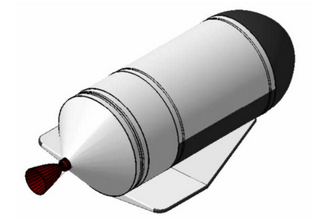
\includegraphics[height=6cm]{greder}
\end{center}
\vspace{0.8cm}
% Author and supervisor
\noindent
\begin{minipage}{0.4\textwidth}
  \begin{flushleft} \large
    \emph{Authors :}\\
    Tim \textbf{\textit{Lewis}}\\
    Alina \textbf{\textit{Trifunovic}}\\
    Lukas \textbf{\textit{Krause}}\\
    Alexis \textbf{\textit{Rolin}}\\
    Julien \textbf{\textit{Huynh}}\
  \end{flushleft}
\end{minipage}%
\begin{minipage}{0.4\textwidth}
  \begin{flushright} \large
    \emph{Supervising professor :} \\
    Prof. Dr.-Ing. Uwe \textit{Apel}\\
  \end{flushright}
\end{minipage}

\vfill

% Bottom of the page
{\large Version 1.0.1\\ \today}

\end{center}
\end{titlepage}

%%%%%%%%%%%%%%%%%%%%%%%%%%%%%
%%% Non-significant pages %%%
%%%%%%%%%%%%%%%%%%%%%%%%%%%%%

\frontmatter

%\chapter*{Remerciements}


\tableofcontents

\mainmatter
\pagestyle{fancy}
%%%%%%%%%%%%%%%%%%%%%%%%%%%%%%%%%%%%%%%%%%%%
%%% Content of the report and references %%%
%%%%%%%%%%%%%%%%%%%%%%%%%%%%%%%%%%%%%%%%%%%%



\chapter{Introduction}
\chapter{Schedule}

\qquad At the start of the project a dedicated group meeting was performed in order to agree on a common project sequence, tasks and challenges as well as work distribution. This group meeting was deemed essential to structure the work packages and to achieve a consolidated baseline for the whole project including time line.\\

The result is a complex MS project Gantt diagram, which can be found in \nameref{sec:annex1}.\\
\section{Initial Schedule}
\qquad The first version of the schedule starts with a project Kick-Off in October which is afterwards followed by a short planning phase. In this planning phase issues as scheduling, work distribution and scope of the project were addressed.\\

Subsequently, the definition phase started. Within this phase, the vehicle requirements were defined and the mission was planned, calculated and visualized in MATLAB. The outcomes of the definition phase are the boundary requirements which are set to provide a frame for both: the vehicle itself as well as the propulsion system. The requirements were defined at the beginning of the project and were verified after project completion.\\

Upon definition of the boundary requirements, the specification phase started. Within this phase, different propellant combinations were identified, discussed and compared. Additionally a first mass budget was calculated. The result of this phase is the system specification.\\

The sequence of the project includes several presentations. The first one was performed in October for a quick overview on the project planning. The second one after the boundary requirements and system specification was set. 
After this presentation, the vehicle and sub system design phase started. This phase included major parts of the work packages including propulsion system design with all sub-assemblies as RACS/ACS, propellant tanks, feeding and pressurization system, turbo pumps, catalyzer, engine, injector and nozzle. The outcome of this phase is a preliminary vehicle design and sub system design which was presented in the mid-term presentation.\\

As a last major work package the simulation phase started. The whole system was simulated including all sub systems and additionally the complex H2O2 decomposition regulation. The final presentation was performed after all tasks were completed and the simulation was finalized.\\

An overview the compressed initial schedule is shown in \autoref{Fig1}. The detailed Gantt schedule can be found in Annex 1.

\begin{figure}[H]
	\centering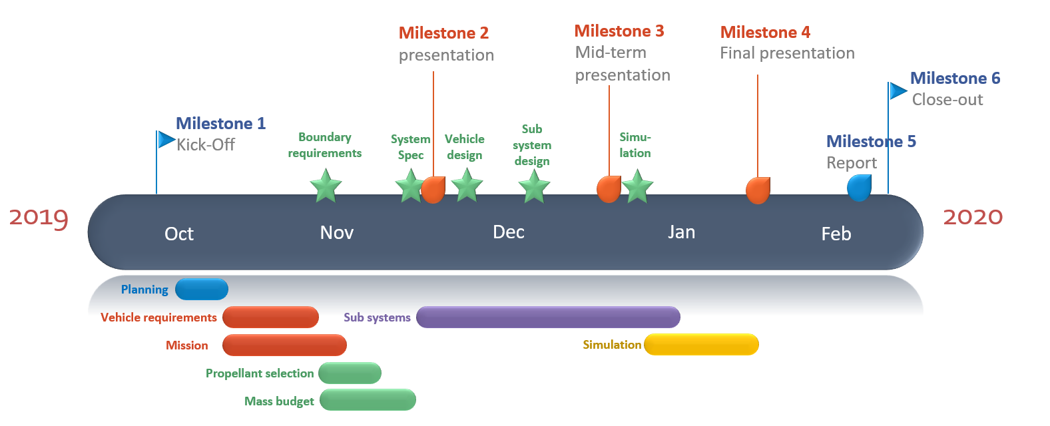
\includegraphics[width=\linewidth]{initialschedule}
	\caption{Initial schedule}\label{Fig1}
\end{figure}

\section{Final schedule – comparison as planned and as achieved}

\qquad As usual in project management and project work, not all milestones were achieved in time. As it is shown in the compressed final schedule in \autoref{Fig2}, the finalized vehicle design, the finalized sub system design and the corresponding simulation shifted within the project schedule (\autoref{Fig2}, shown in red). Nevertheless all work packages have been successfully completed until Milestone 4, the final presentation.

\begin{figure}[H]
	\centering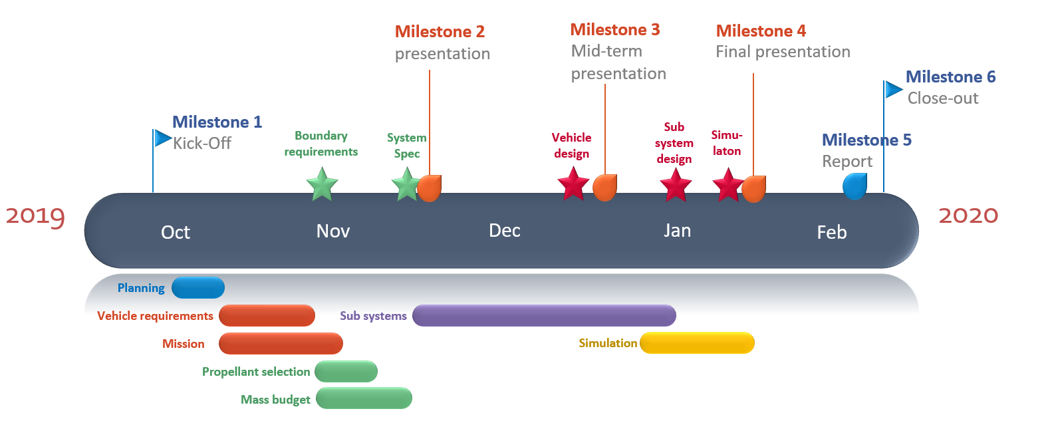
\includegraphics[width=\linewidth]{finalschedule}
	\caption{Final schedule - comparison as planned and as achieved}\label{Fig2}
\end{figure}


\chapter{Requirements}
\qquad The top level requirements for the vehicle and propulsion system are divided in three categories: operation, environment and vehicle. The operation requirements are related to the propulsion system and its applicability for the planned missions. The environmental requirements are defined to ensure that both the vehicle and propulsion system is capable of operating and sustaining during launch, mission and in space environment. The scope of the vehicle requirements is to cover the major parts of the planned mission as refuel-ability, aero braking or accuracy. \\
\noindent
\begin{table}
\begin{tabular}{|c|}
	\hline
	\cellcolor{blue!60}\textbf{Operation}\\
	\hline
	\cellcolor{blue!15} TL-1 Provide sufficient thrust for completion of the mission profile including a safety margin\\
	\hline
	\cellcolor{blue!15} TL-2 Re-ignitable at least 1000 times\\
	\hline
	\cellcolor{blue!15} TL-3 Service life time of at least 100 missions or 25 years in orbit\\
	\hline
	\cellcolor{blue!15} TL-4 Ignition and functional reliability shall be higher than 99,5\%\\

	\hline
	\cellcolor{blue!60}\textbf{Environment}\\
	\hline
	\cellcolor{blue!15} TL-5 Withstand the launch phase
	\\
	\hline
	\cellcolor{blue!15} TL-6 Operate in vacuum
	\\
	\hline
	\cellcolor{blue!15} TL-7 Operate in an ambient temperature range of 1K to 5K
	\\
	\hline
	\cellcolor{blue!15} TL-8 Withstand the temperature gradients resulting from areas turned towards or away
	\\
	\hline
	\cellcolor{blue!15} TL-9 Sustain space-related radiation throughout it's complete life time
	
	\\
	\hline
	\cellcolor{blue!15} TL-10 Withstand debris impact of under 1cm diameter with a max relative speed of $15$ km/s 	
	\\
	\hline
	\cellcolor{blue!60}\textbf{Vehicle}\\
	\hline
	\cellcolor{blue!15} TL-11 The engine shall be the main propulsion system of a GEO satellite recovery vehicle
	\\
	\hline
	\cellcolor{blue!15} TL-12 Refuelable between missions
	\\
	\hline
	\cellcolor{blue!15} TL-13 Perform aerobrake maneuvers in Earth's atmosphere.
	\\
	\hline
	\cellcolor{blue!15} TL-14 Control \space flight path in  Earth's atmosphere  using non-propulsive flight control systems
	\\
	\cellcolor{blue!15} TL-15 Remain within the ARIANE 6/Falcon 9 payload launch capabilities to LEO.
	
	\\
	\cellcolor{blue!15} TL-16 Remain on it's guided trajectory with less than 0.1\% deviation.
	
	\\
	\hline
\end{tabular}
\caption{Requirements for the vehicle}
\end{table}
\chapter{Launcher requirements and launch envelope}

From our initial requirements we set to stay within certain margins of size and mass. These two parameters create constraint for the launch. 
Indeed, we have to analyze the different launcher on the market and their capabilities. 
Thus, we chose to stay within the capabilities of two of the most used actual launchers: Ariane 6.4 and Falcon 9. \\

These launchers have almost the same launch capability; the Falcon 9 can send $22.8$ t in LEO and Ariane 6.4 can send $21.6$ t to LEO.
The other important characteristic is the dimension of the fairing.
Here we have two different launchers with almost identical size; the Falcon 9 can carry a payload up to $11.4$ m long and $4.6$ m wide, whereas Ariane 6.4 can carry up to $18$ m long and $4.57$ m wide but as the Ariane's fairing is very elongated the true usable size will be more around $12$ m by $4.57$ m. \\

To allow us to correctly design our spacecraft we need to create a theoretical envelope based on these two launchers. For that we set the following dimension: a diameter of $4.5$ m and a total length of $11.4$ m. These dimensions are lower than the two launchers to unsure to have a safety margin.

\clearpage

To sum up, here is the 3 fairing we spoke about:

\begin{figure}[H]
    \centering
    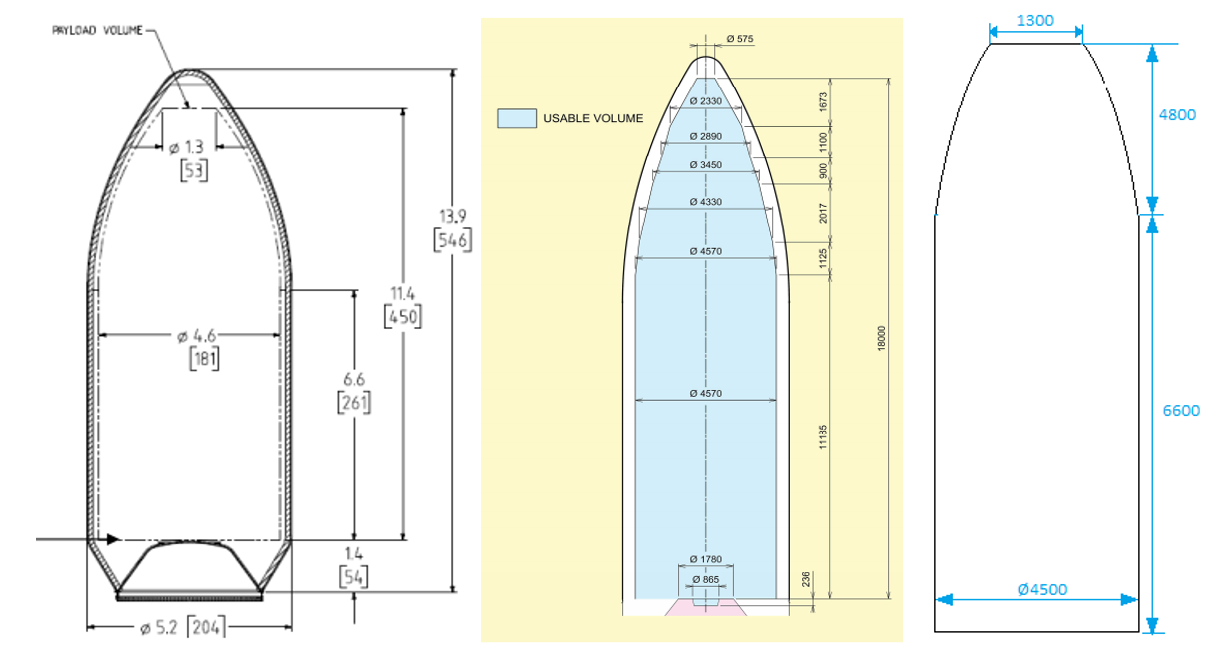
\includegraphics[width=\linewidth]{enveloppe}
    \caption{Falcon 9 - Ariane 6 - combined fairing}
    \label{fig:my_label}
\end{figure}

In case, during the design process, the spacecraft cannot stay behind the 22t to LEO launch capability of the Falcon 9, we plan to use the bigger Falcon Heavy which can send 60t to LEO. This launcher will be the last choice, we want at most to stay within our pre-requirement. \\

We first think to use the structure of our spacecraft, which is aerodynamic, as a fairing so we have less constraint on the size but as it has wings and tail it will generate a small lift but sufficient to destabilize the launcher and might cause a crash. So we decided to forget this idea and to stay within a classic fairing. \\

Through our project we are going to see if our requirements can meet our calculations and we will make a choice of launcher. 
\chapter{Mission analysis}
\qquad \underline{By} : Tim
\section{Mission Summary}
The objective of the mission is the deorbiting of a GEO satellite. The first step to developing the
propulsion system is to break down the mission segments and calculate the delta-V for each of them.
Then after the $\Delta v$ and some mission constraints are clear the detailed mission profile needs to be chosen and optimized.\\

The mission is broken down into two major phases. Phase 1 is to reach the satellites orbit and match its
velocity to enable the capturing process. Phase 2 is deorbitng te satellite and retuning to the original LEO orbit.
\subsection{Phase 1}
\begin{center}
	Transferring the spacecraft from LEO at $55^\circ$ inclination to GEO at $0^\circ$ inclination
\end{center}
First concept : \\

\begin{itemize}
	\item Burn 1.1 : LEO to GTO at $55^\circ$
	\item Burn 1.2 : Inclination change to $0^\circ$ at Apogee of GTO
	\item Burn 1.3 : GTO to GEO at $0^\circ$
\end{itemize}
To calculate the required delta-V for a burn to change the velocity without changing the direction of the spacecraft is simply identifying the difference in value of the starting and target vector. So for Burn 1.1 the orbital speed of LEO at 400 km needs to be calculated as well as the perigee speed of an elliptic orbit with 400 km as perigee and GEO altitude as apogee. To calculate these values several Matlab functions were written:

\begin{minted}[fontsize=\footnotesize, linenos, autogobble, breaklines]{matlab}
function a = v(r) % velocity of a circular orbit with Radius r
a = sqrt(mu/r);
end
\end{minted}
Then the function was used for the calculation with $R_{LEO} = 6778$ km
\begin{equation}
	v_{LEO} = v(R_{LEO}) = 7669 m/s
\end{equation}
The target velocity for the perigee of the GTO is calculated with the following function:
\begin{minted}[fontsize=\footnotesize, linenos, autogobble, breaklines]{matlab}
function a = vp(r, R) % perigee velocity of elliptical orbit with perigee r and apogee R
if r<R %if clause to prevent mistaken input
a = sqrt(2*mu/r-2*mu/(r+R));
end
end
\end{minted}

With $R_{GEO} = 42164$ km, the speed is calculated:
\begin{equation}
	v_{gto_p} = v_p(R_leo, R_geo) = 10066 m/s
\end{equation}
The difference between the two values is the required $\Delta v, \Delta v_1 = 2398$ m/s.\\

To calculate the delta-V needed for an inclination change the following function was used:
\begin{minted}[fontsize=\footnotesize, linenos, autogobble, breaklines]{matlab}
function a= dVi(i, v) % delta-V required for inclination change of i (deg) and velocity v
a= 2*v*sin(deg2rad(i)/2);
end
\end{minted}

The velocity passed to the function is the velocity at which the inclination change shall be performed.
Here the apogee velocity of the GTO $v_{gto_a} = 1618$ m/s was used:
\begin{equation}
	\Delta v{inc_1} = \Delta v_i(i, v_{gto_a})
\end{equation}

Lastly, the velocity change from the apogee of the GTO $v_{gto_a}$ and the velocity at GEO $v_{geo} = 3075 m/s$ needs to be calculated. The difference between the two values is $\Delta v_2 = 1457$ m/s.\\

Now all the three delta-Vs are added to the delta-V requirement of phase 1:
\begin{equation}
	\Delta v_{phase_1} = \Delta v_1+\Delta v_1+\Delta v_{inc1} = 5348 m/s
\end{equation}


\subsection{Phase 2 }
\begin{center}
	Transferring the captured satellite to a deorbiting trajectory and returning to LEO at $55^\circ$ inclination
\end{center}
First concept : \\


After capture the satellite needs to be deorbited. Herefore it needs to be set to a drop trajectory. But
since the spacecraft shall not deorbit but stay in LEO it needs to make short correction burn to slightly increase the targeted perigee.
\begin{itemize}
	\item Burn 2.1 : GEO to GTO with (with DROP altitude as perigee, afterwards detaching the satellite)
	\item Burn 2.2 : Inclination change to $55^\circ$
	\item Burn 2.3 : GTO(DROP) to GTO(LEO as perigee)
	\item Burn 2.4 : GTO(LEO) to LEO
\end{itemize}
These $\Delta v$ are calculated in the same way as described above. The total $\Delta v$ for phase 2 with $v_{drop_a} = 1587$ m/s, $v_{aero_{a1}} = 1592$ m/s, $v_{aero_{p1}} = 10283$ m/s, $v_{lto_p}
= 7887$ m/s and $v_{lto_a} = 7596$ m/s.

\begin{align}
	\Delta v_3 &=\Delta v(v_{GEO}, v_{drop_a}) = 1488 m/s\\
	\Delta v_4 &=\Delta v(v_{drop_a}, v_{aero_{a1}}) = 5 m/s   \\
	\Delta v_5 &=\Delta v(v_{aero_{p1}}, v_{lto_p}) = 2396 m/s   \\
	\Delta v_{inc_2} &=\Delta v_i(i, v_{drop_a}) = 1465 m/s   \\
	\Delta v_6 &=\Delta v (v_{lto_a}, v_{leo}) = 72 m/s  \\
	\Delta v_{Phase_2} &= \Delta v_3 + \Delta v_4 + \Delta v_{inc_2} + \Delta v_6 =3031 m/s
\end{align}
Since this maneuver is very costly in terms of fuel consumption the concept of aerobraking was
introduced. An aerobrake is using the atmospheric drag in the upper atmosphere to brake and reduce
velocity. For this mission an aerobrake can save a large amount of delta-V and fuel respectively. in that case, $\Delta v_5$ does not need to be included in the sum, saving 2396 m/s.

\section{Delta-V reduction}
There are further means which enable the reduction of delta-V. The ones applied will be discussed in the
following.\\

\textbf{\underline{Combining burns}}\\
It can make sense to combine burns. Since Inclination changes require burns perpendicular to the flight
direction they can be combined with accelerating or decelerating burns in flight direction. The resulting vector is of shorter length than the sum of the separate burns. Thus, less fuel needs to be burnt. To combine inclination and velocity changing burns the following function was used:
\begin{minted}[fontsize=\footnotesize, linenos, autogobble, breaklines]{matlab}
function a = cosl(v1, v2, i) % combined maneuver of velocity change v1 -> v2 and inclination i change
a = sqrt(v1^2+v2^2-2*v1*v2*cos(deg2rad(i)));
end
\end{minted}

The function uses the Cosine-law to calculate the magnitude of the vector between the original velocity
vector and the target vector rotated by the required inclination.\\

\textbf{\underline{Splitting inclination change burns}}\\
Mostly it makes most sense to make the inclination change at the lowest possible velocity, since the
velocity vector needs to be rotated and this is easier with a shorter vector. However, when the inclination change is split up to combine with further necessary burns the fuel consumption be reduced even further. For the GREDER spacecraft the burns were optimized to reduce the $\Delta V$ to the lowest feasible. The outcome of various optimization loops was to split the inclination change into $1.7^\circ$, $52.6^\circ$ and $1.7^\circ$ as shown in \autoref{tab:missionoption} below.\\

\textbf{\underline{Overshooting the apogee for inclination change}}\\
Since the inclination change is most efficient at lowest velocities it can make sense to overshoot the
targeted apogee and adding a burn to reach the targeted orbit with the inclination already changed. The
inclination change is then performed combined with the added burn to get to the originally targeted orbit.\\

Compare options 3 and 5 in the \autoref{tab:missionoption} below. The higher the orbit the lower is the required $\Delta v$.
However, since increasing the apogee by too much could result in reaching the sphere of influence of the
moon and also increase the mission duration by more than tolerable. Also, the increments by which the
delta-V decreases get smaller by a constant increase of apogee. So as a compromise roughly double the
altitude of GEO was chosen at an orbit radius of 90000 km.\\

\textbf{\underline{Inclination change during aerobrake}}\\
Atmospheric drag can help in reducing the velocity of a spacecraft. In addition, it can be used to generate lift and if directed in the right direction this can reduce or even replace a necessary inclination change burn. An aerobrake strongly influences the architecture of a spacecraft though, since some kind of heat shield is mostly necessary. This is discussed in Chapter 6. Also adding wings to the spacecraft increase its mass and structural behaviour.\\

To estimate the best mission profile several different combinations of these strategies were calculated
and compared to each other. The following \autoref{tab:missionoption} shows the considered missions, the number of burns as well as the total necessary delta-V. To reach the best possible delta-V all the different optimization concepts of the team members were taken into account and combined to settle for a final mission profile.


\begin{table}
	\begin{tabular}{|c|c|c|c|c|}
		\hline
		Option & Phase 1 & Burns & $\Delta v$ (km/s) & Remarks\\
		\hline
		1 & LEO - GTO - INC55 - GEO & 3 & 5.3483 & \\
		\hline
		2 & LEO - GTO - INC55/GEO & 2 & 4.9203 & \\
		\hline
		3 & LEO - INC3/GTO - INC52/GEO & 2 & 4.8796 & \\
		\hline
		4 & \makecell{LEO - LEOto90k -\\ INC55 - 90ktoGEO - GEO} & 4 & 4.9241 & \\
		\hline
		5 & \makecell{LEO - LEOto90k -\\ INC55/90ktoGEO - GEO} & 3 & 4.6916 & \\
		\hline
		6 & \makecell{LEO - INC1.7/LEOto90k\\ - INC51.6/90ktoGEO - INC1.7/GEO} & 3 & 4.6674 & \\
		\hline
		7 & \makecell{LEO - LEOto90k - INC55\\ - 90ktoAERO - AEROtoGEO - GEO} & 5 & 5.0133 & \\
		\hline
		8 & \makecell{LEO - LEOto90k - INC55/90ktoAERO\\ - AEROtoGEO - GEO}  & 4 & 4.9935 & \\
		\hline
		& Phase 2 & & & \\
		\hline
		9 & \makecell{GEO - GEOtoDROP - INC55\\ - GEOtoAERO - AEROtoLEO} & 4 & 3.0309 & \\
		\hline
		10 & \makecell{GEO - GEOtoDROP\\ - GEOtoAERO - AEROtoLEO} & 3 & 1.5655 & \makecell{\small inclination change\\ \small through aerobrake}\\
		\hline
	\end{tabular}
\caption{Mission planning options}\label{tab:missionoption}
\end{table}

Changing the inclination at the perigee with the highest velocity requires a lot more energy than at GEO
altitude. However, if this is achieved without burning fuel and with a lifting body instead a considerable amount of fuel and $\Delta V$ is saved. This resulted in the team decision to settle for the combination of option 6 and 10. The complete mission $\Delta v$ is composed by the following parts:\\
\textbf{\underline{Phase 1}} :
\begin{itemize}
	\item $\Delta v = 4.67$ km/s
\end{itemize}
{\underline{Phase 1 savings}} :
\begin{itemize}
	\item Combined burns : $\approx 430$ m/s
	\item Overshooting the apogee : $\approx 230$ m/s
\end{itemize}
\begin{figure}[H]
	\centering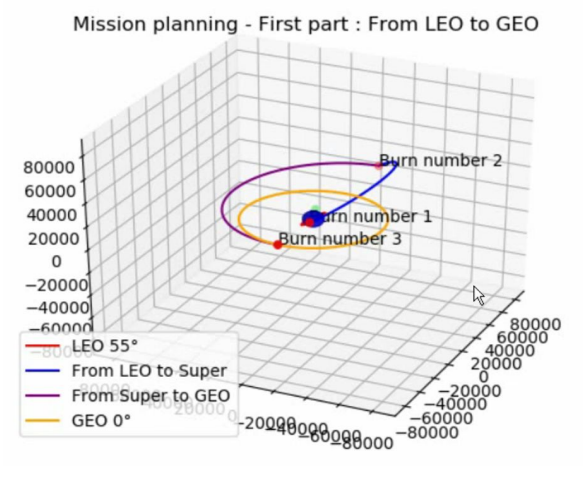
\includegraphics[width=0.6\linewidth]{mission1}
	\caption{Mission planning - First part}
\end{figure}
\textbf{\underline{Phase 2}} :
\begin{itemize}
	\item $\Delta v = 1.57$ km/s
\end{itemize}
{\underline{Further secondary burns}} :
\begin{itemize}
	\item Steering, rotation : $\approx 80$ m/s
	\item Reserve, correction : $\approx 200$ m/s
	\item Capture : $\approx 100$ m/s
\end{itemize}
\underline{\textbf{Total $\Delta v$ for the whole mission}} : $6.61$ km/s
{\underline{Phase 2 savings}} :
\begin{itemize}
	\item Aerobrake : $\approx 390$ m/s
	\item Inclination change during aerobrake : $1470$ m/s
\end{itemize}
\underline{\textbf{Total savings in both phases}} : $2.95$ km/s\\

\autoref{figtim2} shows the paths of the second part of the mission. Here only one exemplary aerobrake orbit is shown as a simplification.
\begin{figure}[H]
	\centering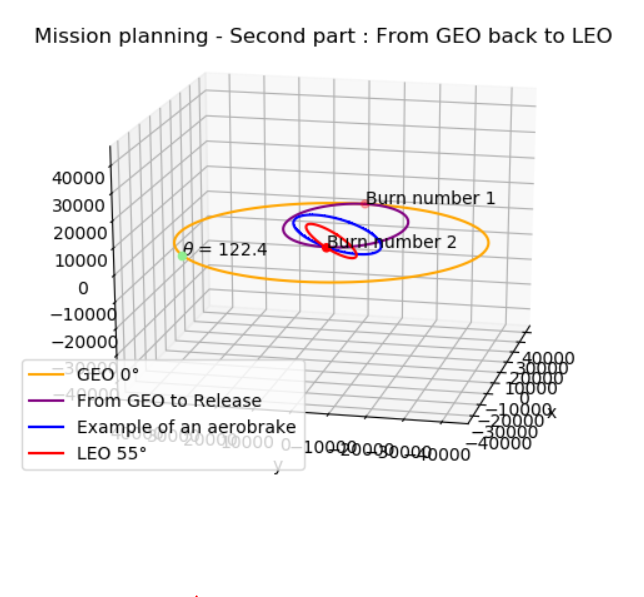
\includegraphics[width=0.7\linewidth]{mission2}
	\caption{Mission planning - Second part}\label{figtim2}
\end{figure}
\chapter{Satellite catching process}
\label{sec:5}
\section{Choice of the process}

\qquad In order to catch and de-orbit a satellite in GEO, we considered the following usable tools :
\begin{itemize}
	\item Net
	\item Harpoon
	\item Claw
	\item Magnet
\end{itemize}

Other solutions such as towing the satellite or simply removing them from GEO were not considered as they either did not fit our program or would create too much strain on our spacecraft.\\

We then took a closer look at the feasibility of each solution and compared the advantages and disadvantages :
\begin{center}
	\begin{tabular}[H]{|c|c|c|c|}
		\hline
		\textbf{Solution} & \textbf{Advantages} & \textbf{Drawbacks} & \textbf{Feasibility}\\
		\hline
		\textbf{Net} & Cheap, simple, low mass &Slow, hard to handle & Yes (JAXA, ESA)\\
		\hline
		\textbf{Harpoon} & Fairly cheap & Can create more debris& Yes (ESA)\\
		\hline
		\textbf{Claw} & Safer & Mechanical, moving parts& WIP (CleanSpace One)\\
		\hline
		\textbf{Magnet} &Adjustable, no moving parts & Higher mass, needs power& Research State\\
		\hline
	\end{tabular}
\end{center}

As the main focus of our mission is reliability and re-usability, we made the choice of using magnets to catch and hold the satellite we would like to de-orbit.

\section{Magnetic solution}
\qquad Even though we decided that we would use magnets, we needed to make sure it was feasible and to lower the drawbacks related to this solution as much as possible. The first precision we need to make is that we will be using electromagnets in order to regulate the intensity of the current in the coil of it, thus, modulating the attraction force so the contact between our spacecraft and the satellite will not be made at high velocity, avoiding damages and space debris creation. \\

Even though it is still at the state of research, we believe that using electromagnets as our catching solution is realistic as both ESA (with ISAE SupAero) and the NASA have been considering and studying this solution since 2017.\\

However, as a matter of complexity, we will have to make assumptions in order to simplify the problem. The objective in this part is to prove that, with assumptions, this solution can be applied to our mission and to find the required energy to both catch and hold the satellite until its release.
\subsection{Assumptions}
In our calculations, we assumed that :
\begin{enumerate}
	\item We can consider the magnetic circuit between GREDER and the nozzle of the satellite is a closed one (no air gaps)
	\item About $0.1$\% of the satellite's mass is magnetically operable
	\item Mutual attraction is relatively low compared to the magnetic force
	\item Residuals in the alloy of the magnets' cores are neglectable
\end{enumerate}
\section{Sketching and Calculations}
Using the first assumption, we can use the formula for the magnetic force in a magnetic circuit with no air gap :
\begin{equation}
F = \frac{(\mu NI)^2 A}{2\mu_0 L^2}
\end{equation}
With : 
\begin{itemize}
	\item $\mu$ the magnetic permeability of the core of our magnet (determined by the alloy)
	\item $N$ the number of turns of the coil around the core
	\item $I$ the current running through the coil
	\item $A$ the cross section area of the core
	\item $\mu_0$ the magnetic constant
	\item $L$ the length of the mean magnetic circuit
\end{itemize}
In order to have a good balance between thermal properties and magnetic properties we decided to use an alloy made of $90$\% of iron and $10$\% of cobalt for our core. We decided to use this alloy as iron has the best magnetic properties (high relative magnetic permeability) and added cobalt as it has a higher Curie Temperature than iron but has a lower relative magnetic permeability.

In terms of magnet design, we chose to use a squared cross section of $5cm\times 5cm$ for the magnet core and with a length of $15cm$, made of an iron-cobalt alloy and a copper coil around it. We decided to have $135$ turns of the coil around the core with a coil diameter of $1mm$ in order to not have the wire revolutions stuck to each other. We also want to run a current of $10A$ through the coil.\\

\begin{figure}[H]
	\centering
	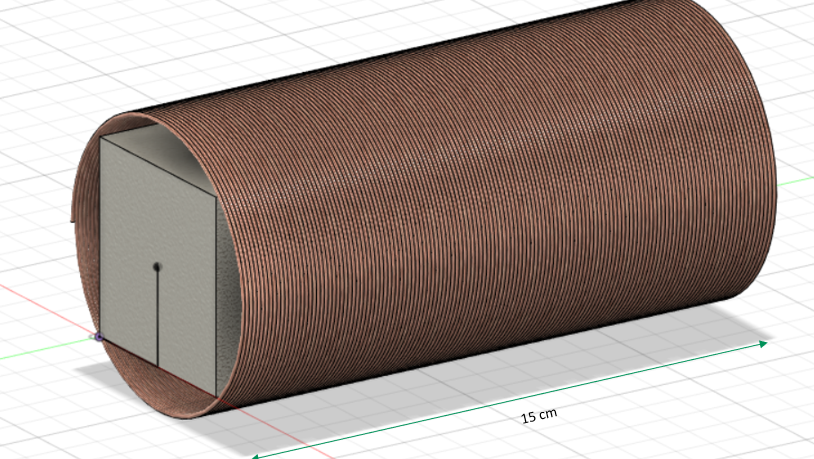
\includegraphics[width=\linewidth]{magnetCAD}
	\caption{CAD of a catching magnet}
\end{figure}


With those design choices we get the following parameters while taking into consideration that there should not be any kind of residuals in the core alloy :

\begin{itemize}
	\item $\mu_0 = 4\pi \times 10^{-7}\ H/m$
	\item $\mu = \bigg(\frac{\mu_{iron}+\mu_{cobalt}}{2}\bigg)\times\mu_0=5.868\times10^{-3}\ H/m$
	\item $N=135$ turns
	\item $I = 10\ A$
	\item $A = 25cm^2=2.5\times10^{-3}\ m^2$
	\item $\rho_{core} = \rho_{iron}\times 0.9 + \rho_{cobalt}\times0.1 = 7.9726\ g/cm^3$
	\item $\rho_{coil} = \rho_{copper} = 8.96\ g/cm^3$
\end{itemize}

We then need to find the length $L$ of the mean magnetic circuit. In order to do so, we decided to start the catching sequence at $10\ m$ from the satellite and that the target has an exploitable nozzle of $40\ cm$ of diameters which is realistic for spacecrafts in the mass range of $3\ 500\ kg$. We could then sketch the catching sequence as so (not to scale) :

\begin{figure}[H]
	\centering
	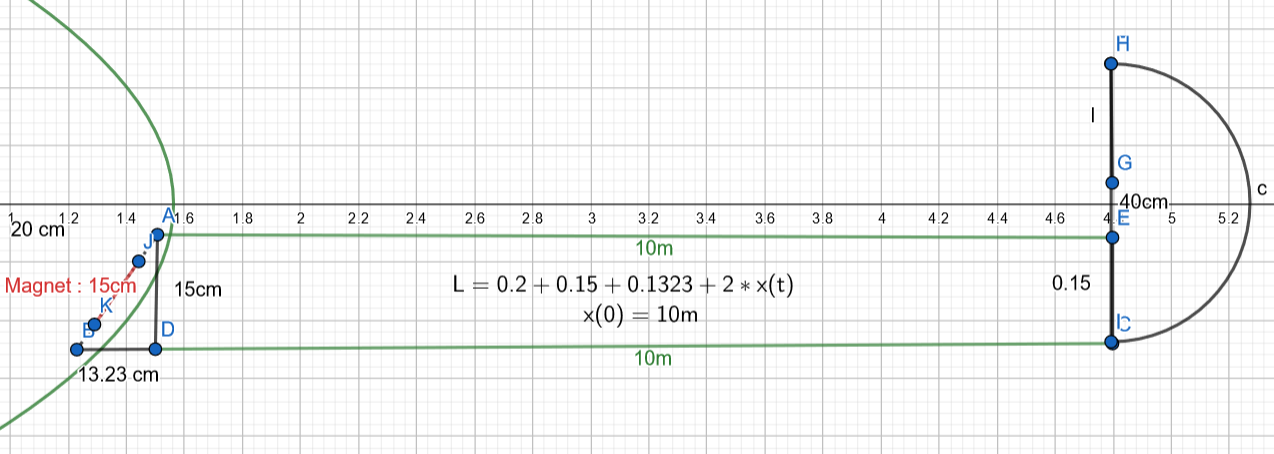
\includegraphics[width=\linewidth]{catching}
	\caption{Catching sequence (not to scale)}
\end{figure}
We can then have the length $L$ as a function of the distance between the tip of our spacecraft and the nozzle of our target. As a result we can proceed to find the feasibility of our solution with this magnet design by finding the time it would require at this state to attract the target. However, in this case, the current modulation when the target is close has not been modeled due to its complexity.\\

Considering that the force will be on one axis only and $m = 0.001\times m_{target} = 3.5\ kg$ :
\begin{align}
\vec F &= m\vec a\\
\frac{(\mu NI)^2 A}{2\mu_0 L(x)^2} &= m \times \ddot x\\
\frac{(\mu NI)^2 A}{2\mu_0 [0.2 + 0.15 + 0.1323 + 2x(t)]^2} &= m \ddot x(t)\\
\frac{(\mu NI)^2 A}{2\mu_0 [0.4823 + 2x(t)]^2} &= m \ddot x(t)
\end{align}

The catching time can then be found using $ode45$ on Matlab :
\begin{minted}[fontsize=\footnotesize, linenos, autogobble, breaklines]{matlab}
clearvars; clc;
catchtime = 1;
x0 = 10;
while 1
    [t,x] = ode45(@f3,[0:1:catchtime], [x0; 0; 0; 0]);
        if (x(catchtime ,1) >= 2 * x0)
            break
        else
            catchtime = catchtime +1;
        end
end
\end{minted}
And the function used for the $ode$ solver :
\begin{minted}[fontsize=\footnotesize, linenos, autogobble, breaklines]{matlab}
function  [Xdot] = f3(t, X)
mu = 5.686e-3; mu0 = 4 * pi * 10 ^(-7);
N = 135; I = 10; A = 0.05 ^ 2; m = 3500 ;
x = X(1); y = X(2); vx = X(3); vy = X(4);
Fmag = (mu * N * I) ^2 * A / (2 * mu0 *(2 * norm(X(1:2)) + 0.4823) ^ 2 );
Xdot = [vx; vy;  0.001 * Fmag / m; 0]; 
end
\end{minted}
We then get a catching time of $812$ seconds. As a result, we can determine the energy required to operate the magnets aswell as their masses and volumes. We are considering a holding time for approximately half an hour and we also need to verify that the magnets will be able to hold the target while we are de-orbiting.
\chapter{Thermal protection system}

\qquad A complete deorbiting mission from LEO to GEO and returning to LEO has a very high delta-V requirement of  roughly $8.5$ km/s. To reduce this delta-V the GREDER spacecraft will use atmospheric drag in the upper atmosphere at an altitude of $70-120$ km to reduce its relative velocity when returning from GEO to LEO. This kind of maneuver is called an aerobrake and has the potential to save a significant amount of fuel and total spacecraft mass. Aerobrakes are commonly used for reentry vehicles. However, these experience very high thermal loads since the kinetic energy is converted to heat through friction with the atmosphere in a single reentry trajectory. Thus, a high mass for a heat shield is necessary. For a reusable spacecraft ablative heat shields are not useful. Instead, a passively cooled thermal protection system (TPS) was chosen. This allows to radiate the heat away. When the velocity is reduced into small increments the spacecraft can radiate the heat away in the time between the aerobrakes. The advantage is, that fuel is only required for trimming maneuvers to set the targeted perigee radius and not for the decelleration itself. A high number of aerobrakes can be performed with relatively small heat loads if extended mission time is not of a large concern.\\

Since the GREDER spacecraft is unmanned and does not utilize cryogenic fuels the extended mission time is not as critical. A heat shield needs to be developed for the spacecraft to protect it at the areas with the highest heat loads.

\section{First estimation}

\qquad For first rough calculations the total velocity reduced by the aerobrakes was determined as $2.4$ km/s. This is the difference in velocity between the perigee velocity of the transfer orbit from GEO to aerobraking altitude and the velocity of the perigee of the transfer orbit from the last aerobrake to LEO. The mass of the spacecraft after deorbiting was estimated at $3500$ kg. This results in a kinetic energy of:

\begin{equation}
	E_{kinetic} = \frac{m_{sc}\Delta v^2}{2} = 10.04\ GJ
\end{equation}

For a number of $15$ aerobrakes this kinetic energy needs to be divided by $15$ assuming the temperature at the beginning of each aerobrake will be the same.  This kinetic energy was then assumed to be completely converted to thermal energy and distributed evenly over the mass of a heat shield. With the maximum allowable temperature of the chosen material a rough required heat shield mass could be estimated.

\section{Material choice}

\begin{align}
	E_{kinetic} &= \frac{mv^2}{2}\\
	m_{shield} &=\frac{E_{kinetic}}{c\times dT}
\end{align}
\begin{table}
	\centering
	\footnotesize
	\begin{tabular}{|c|c|c|c|c|}
		\hline
		Property & \makecell{Reinforced\\ Carbon-Carbon} & \makecell{Aluminium\\ (2024-T8XX)} & \makecell{Steel\\ Type 321} & \makecell{Titanium (6A1-4V)}\\
		\hline
		Density (kg/m$^3$) & $1578$ & $2803$ & $8027$ & $4437$\\
		\hline
		\makecell{Thermal conductivity\\ ($W/m-K$)} & $3.9^*$ & $145.4$ & $14.7$ & $69$\\
		\hline 
		\makecell{Specific heat\\ ($J/kg-K$)} & $711.8$ & $816.4$ & $565.2$ & $523.4$\\
		\hline 
		\makecell{Multipule Use\\ Temperature Limit ($K$)} & $1922$ & $ 425^{**}$ & $872^{**}$ & $662^{ **}$\\
		\hline 
		\makecell{Single Use\\ Temperature Limit ($K$)} & $2033$ & $450$ & $922$ & $700$\\
		\hline
		$T_{cond}\times M_{TempLim} (E+6)$ & $1.41$ & $0.35$ & $0.49$ & $0.35$\\
		\hline 

	\end{tabular}
\vspace*{0.2cm}
 (*thru-the-thickness not isotropic; **values extrapolated by ratio of single/multiple use of CFRC) 
	\caption{Comparison of materials for heat shield}
\end{table}
The table above is a comparison of possible TPS materials. The values are taken from the TPSX NASA Material Properties Database. Multiple Use Temperature values were not available for the chosen metals but were extrapolated based on the ratio of the multiple and single use temperature limits of CFRC. The last row shows the product of the values of the lines Specific Heat and Multiple Use Temperature Limit. This relative value allows to quickly compare the materials with euach other regarding the required mass for a heat shield. The unit is J/kg showing that a high value is favorable to store as much energy as possible per mass.\\

Carbon Fibre Reinforced Carbon quickly proves as the material of choice for a low heat shield mass. Several metals were also taken into account since the manufacturing and integration into the spacecraft struture would be a lot easier. But the low mass for a CFRC TPS in combination with the low thermal conductivity made this the material of choice. CFRC was utilised in the space shuttle heat shield and was found to be the cause of the columbia catastrophe since it is quite brittle and thus sensitive to impact (Columbia Accident Investigation Board Report \footnote{\url{https://www.nasa.gov/columbia/home/CAIB\_Vol1.html}}). But since the GREDER spacecraft will be launched inside a rocket launcher fairing no high velocity impacts are to be expected. The capturing of the satellite on the nose cone will be done at very low relative velocities since the force applied by the magnets is controllable with the applied current and can be carefully adjusted (compare \autoref{sec:5}).
\begin{equation}
	m_{shield_{cc}}= \frac{m_{sc} \times (\Delta v_5\times 1000)^2}{2n_{ab}c_{cc}(T_{max_{cc}}-T_0)}
\end{equation}

With :
\begin{itemize}
	\item $\Delta v_5$ : Required $\Delta v$
	\item $m_{sc}$ : Spacecraft mass
	\item $n_{ab}$ : Number of aerobrakes
	\item $T_{max}$ : Maximum allowable temperature of CFRC
	\item $T_0$ : Temperature at beginning of aerobrakes
\end{itemize}

\section{Lift and drag}

\qquad An aerobrake can also be used to change the inclination of the orbital plane. To achieve this the spacecraft needs to be a lifting body. To increase the lift wings can be attached to increase the projeted area of the spacecraft. This area affects both the lift and drag of the spacecraft.
\begin{align}
	F_l &= C_l\times\frac \rho 2 \times v_1^2 \times A_h\\
	\Rightarrow F_l &= 13.9\ kN\\
	F_d &= C_d\times\frac \rho 2 \times v_1^2 \times A_h\\
	\Rightarrow F_d &= 3.5\ kN
\end{align}

The angle of attack influences the lift and drag coefficients. Since both forces are perpendicular to each other the resulting force and the angle of the direction are calculated by:

\begin{align}
	F_{res} &= \sqrt{F_l^2+F_d^2}\\
	F_{res} &= 14.3\ kN\\
	\beta_{F_{res}} &=\arctan\bigg(\frac{F_l}{F_d}\bigg)\times\frac{180}\pi\\
	\beta_{F_{res}} &=76^\circ
\end{align}

It may be noted that unlike an aircraft the lift vector does not point "upwards" but rather parallel to ground and perpendicular to the orbital plane. Thus, the altitude is not affected by the "lift".\\

The lift and drag coefficient are typically experimental values. For the drag similar shapes can be used as a reference. For the GREDER spacecraft a value of 0.3 is assumed to be reasonable because of its similarity to the bullet shape (compare \autoref{figtim1} and fig xafter). The delta wing should have a significantly lower drag coefficient and is therefore not taken into account.
\begin{figure}[H]
	\centering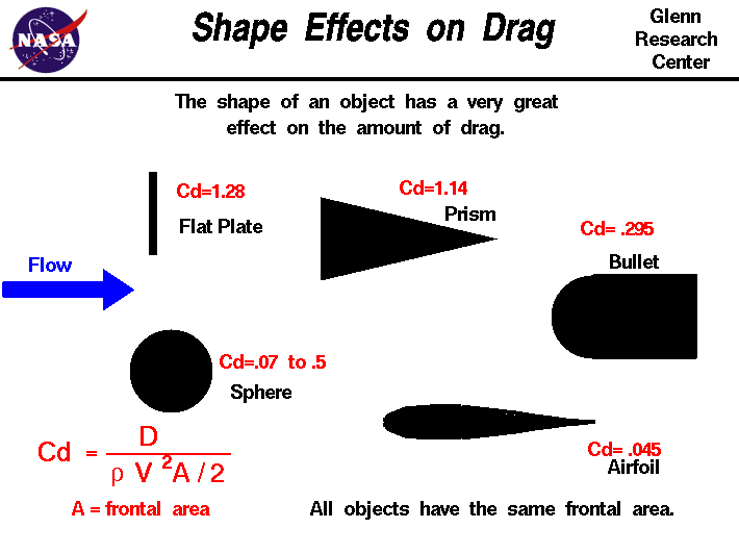
\includegraphics[width=0.7\linewidth]{shapedrag}
	\caption{Shape effect on drag}
\end{figure}

Regarding the lift coefficient a strong simplification as made. For a flat plate the lift coefficient can be approximated with the following formula based on the angle of attack\footnote{\url{http://brennen.caltech.edu/fluidbook/externalflows/lift/flatplateairfoil.pdf}} :
\begin{equation}
	C_L = 2\pi\sin(\alpha)
\end{equation}

For an angle of attack of $11^\circ$ the result for the lift coefficient is $1.2$.\\

To reduce fuel consumption for attitude control a constant angle of attack would be beneficial. To achieve this, the angle between the resulting vector of lift and drag and the velocity vector needs to be the same as the angle between the resulting vector of decelerating and inclination changing vector and the velocity vector. The required delta-Vs for decelerating and inclination change are perpendicular to each other and the angle between them is given by:

\begin{align}
	\beta_{\Delta v_{res}}&=\arctan\bigg(\frac{\Delta v_{inc_{2_p}}}{\Delta v_5}\bigg) = 76^\circ\\
	\beta_{F_{res}} &= \arctan\bigg(\frac{C_L}{C_D}\bigg)
\end{align}

To compute the angle of attack these formulas need to be equated and the formula for $C_L$ included.\\

\begin{equation}
	\alpha = \arcsin(\frac{\Delta v_{inc2_p}}{\Delta v_5}\times \frac{C_D}{2\pi})
\end{equation}

For an angle of attack of $11^\circ$ the angle of the resulting vector of lift and drag is $76^\circ$. This results in a balance of both forces during each aerobrake.

\section{Aerobraking altitude}

\qquad To estimate the altitude of the aerobrakes, the Matlab function atmoscoesa was used. Here the density of the atmosphere is calculated by altitude between $0$ and roughly $84000$ m. The values for higher altitudes are extrapolated. A higher altitude results in a longer necessary time in the atmosphere. This has the benefit of a slower heating up of the spacecraft and low values for lift and drag forces. However this could require a higher number of aerobrakes. Weighing these parameters against each other an altitude of $82$ km was chosen for the aerobrakes. At this altitude the total aerobraking time is $30.4$ minutes. At a number of $20$ aerobrakes each would take roughly 91 seconds. During the first aerobrake the distance traveled would be roughly $937$ km and during the last roughly $730$ km. The forces acted upon the spacecraft are $13.9$ kN for lift and $3.5$ kN for drag. At a remaining scpacecraft mass of $3000$ kg this adds up to an acceleration of $4.8$ km/s$^2$ so roughly $0.5$ Gs. These values seemed reasonable since this would keep the mechanical stress relatively low allowing for reusability of the GREDER spacecraft.

\section{Simplifications}
\qquad Regarding the thermal loads on the spacecraft the heat shield needs a little more detail. Modeling the heat flux and conductance within the heat shield is simplified due to complexity. Since the even distribution of the heat over the shield is inaccurate several conservative assumptions shall leave a margin for this. CFRC retains its mechanical properties up to $2400^\circ$ C\footnote{\url{https://www.makeitfrom.com/material-properties/Carbon-Carbon}}. The maximum allowable temperature used for the heat shield modeling is 2000 Kelvin. Also, the assumed temperature at the beginning of the aerorakes is $400$ Kelvin. Furthermore It is assumed that the entire kinetic energy is converted to thermal energy and this is completely distributed onto the spacecraft. In reality however not only the spacecraft but also the atmosphere would be heated through friction. This is highly dependent on the geometry of the body. Most reentry vehicles use blunt front faces to "push" a protective shock wave heat shield in front of them. This keeps the highest heat loads away from the surface. This affect can be seen in \autoref{figtim1} below. \\
\begin{figure}[H]
	\centering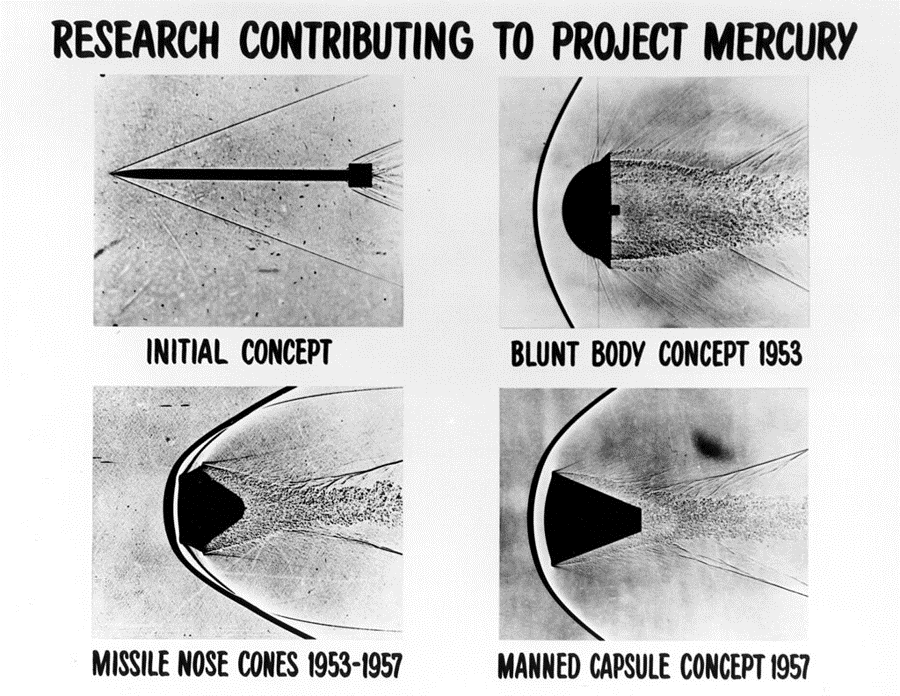
\includegraphics[width=\linewidth]{shadowgraph}
	\caption{Shadowgraph images of Reentry vehicles}\label{figtim1}
\end{figure}

As a further simplification, heat transfer is considered solely through convection during the aerobrake maneuver and solely through radiation during the completion of each orbit. The short duration of the aerobrakes is not very significant compared to the duration of a completed orbit ($90$ s vs. roughly $90$ minutes). Furthermore the heat capacity of CFRC increases with increasing temperature. At $750$ Kelvin the specific heat capacity is roughly double the value compared to ambient temperature (Specific Heat of Carbon/Carbon Composites \footnote{\url{https://apps.dtic.mil/dtic/tr/fulltext/u2/a106709.pdf }}) This leaves an increased margin during the peak heat loads of the atmospheric breaking.

\section{Heat shield interface}

\qquad To avoid mechanical failure of the spaceraft's hull beneath the heat shield an insulating blanket will be applied underneath the CFRC heat shield. Herefore, the flight proven AFRSI Blanket was chosen due
to its excellent isolating properties and very low density. Here a 10 mm layer of the silica blanket at a density of $\rho_AF = 9.6$ kg/m$^3$ and an additive aereal weight of $m_add = 1$ kg/m$^2$ is utilized.\footnote{\url{https://tpsx.arc.nasa.gov/material.html?matid=12}}

The thermal loads are expected to be highest on the leading edges of the spacecraft's wings and the nose of the spacecraft. In these areas the heat shield shall have the largest thickness. \autoref{figtim1} shows the areas where the heat shield will be applied. roughly half of the GREDER spacecraft will be covered by the heat shield. This includes the lower faces and leading faces. The upper side and rear of the spacecraft is not expected to endure high thermal loads during the aerobraking maneuvers since the nose will be tilted upwards exposing the lower side.

\section{Radiative cooling}
\qquad To verify that the radiative cooling of the CFRC shield is sufficient, an interactive model of the radiated heat was created. To calculate the Power radiated by a gray body in space the following formula was used:
\begin{equation}
	P = Aj^* = A\varepsilon\sigma T^4
\end{equation}

The emissivity of CFRC is $\varepsilon = 0.78$ and $\sigma$ is the Stefan-Boltzmann constant. \footnote{\url{https://tpsx.arc.nasa.gov/material.html?matid=24\&units=si}}As a starting
temperature the maximum allowable temperature of $1982$ K was used and for the simulation time the
period of the shortest and last orbit with a period of roughly $80$ minutes or $4800$ seconds. The surface area of the heat shield is half of the total spacecraft surface area.\\

Calculating the emitted energy could be transferred into a temperature delta for each second of the
simulation. after $4800$ iterations the temperature is plotted. The last value of $233$ K is lower than the assumed $400$ K and thus leaves some safety margin.

\begin{minted}[fontsize=\footnotesize, linenos, autogobble, breaklines]{matlab}
sigma=5.6703E-8 %W/m2K4 stefan boltzmann constant
eps_cc=0.78;
T1=zeros(1,4800); %K
T1(1)=1982; %K
for k=1:1:length(T1)-1
T_rad=sigma*T1(k)^4*eps_cc*A_sc_tot/2/c_cc/m_tps_cc;
T1(k+1)=T1(k)-T_rad;
end
plot(T1);
\end{minted}
\begin{figure}[H]
	\centering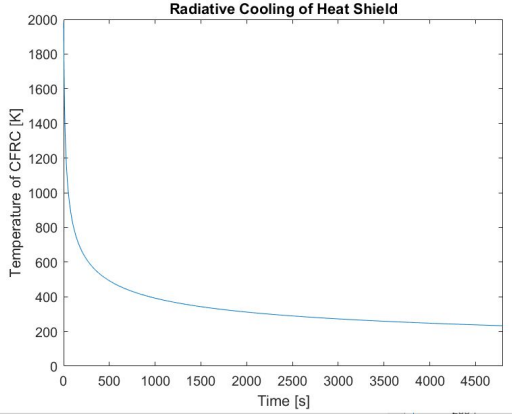
\includegraphics[width=0.9\linewidth]{radcooling}
	\caption{Radiative cooling of the heat shield}
\end{figure}

\section{Final heat shield mass}

\qquad For the final mass of the TPS a specific heat capacity for CFRC of $c_{cc} = 840$ kJ/kg-K was assumed. Moreover :

\begin{itemize}
	\item $\Delta v_5=2.396$ km/s
	\item Spacecraft mass $m_{sc}=3000$ kg
	\item Number of aerobrakes $n_{ab}=20$
	\item Maximum allowable temperature $T_{Max_{cc}} = 1982$ K
	\item Starting temperature $T_0=400$ K
\end{itemize}
At a surface area of the total spacecraft of $A_{sc_{tot}} = 67.4$ m$^2$ and half of the
surface covered with the TPS also the AFRSI blanket mass can be calculated.

\begin{align}
	m_{tps_{cc}} = \frac{(\Delta v_5\times 1000)^2m_{sc}}{2n_{ab}c_{cc}(T_{max_{cc}} - T_0)} = 323.9\ kg\\
	m_{blanket}=\frac{\rho_{AF}A_{sc_{tot}}}{2*0.01} + \frac{A_{sc_{tot}}}{m_{add}} = 37\ kg\\
	m_{tps} = m_{blanket} + m_{tps_{cc}} = 360.9\ kg
	%m_{shield_cc} &= \frac{m_{sc} \times (\Delta v_5\times 1000)^2}{40\times c_{cc}(T_{max_{cc}}-T_0)} = 344.9\ kg\\
	%m_{aerogel} &= A_v\times 0.01\times 200 = 17.3kg\\
	%m_{shield_{total}} &= 362.2 kg
\end{align}
\begin{figure}[H]
	\centering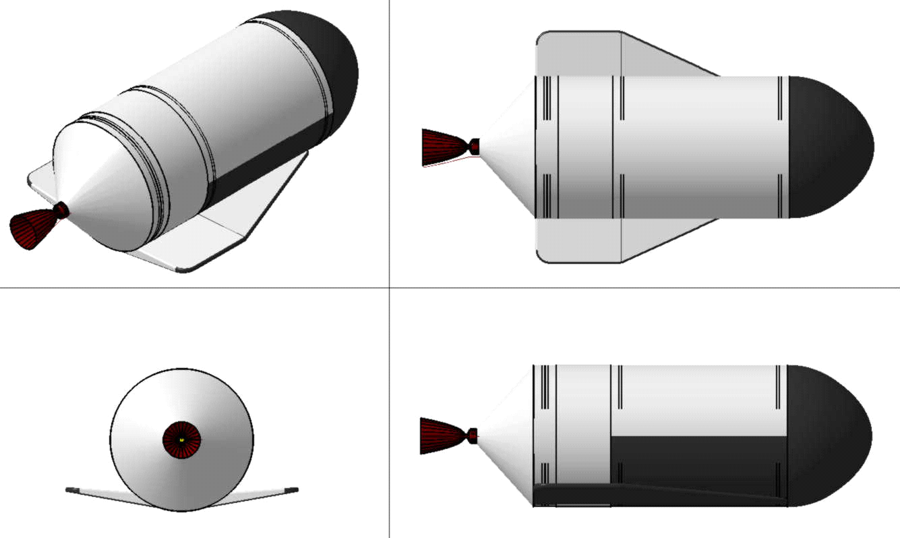
\includegraphics[width=\linewidth]{grederviews}
	\caption{GREDER Spacecraft (various views) - Heat shield sown in gray}
\end{figure}
\chapter{Propellant selection}
\qquad \underline{By} : Alina\\

For the propellant selection for our vehicle, several important aspects have to be taken into account including:
\begin{itemize}
	\item 	Specific impulse in vacuum (Isp) of the propellant
	\item	Storability
	\item	Toxicity including ground handling
	\item	Costs (while the main cost driver is not the propellant itself more its toxicity)
	\item	Reasonable refueling options due to the desired mission profile of the vehicle
	\item	Space flight heritage of the propellant (e.g. flight proven, ground proven or in development)
	\item	Density specific impulse
	\item	Corrosive behavior and compatibility with typical light weight tank materials as titanium or aluminum
	\item	and many more
\end{itemize}

At first several possible and typical flight proven propellant combinations were analyzed and the most promising combinations were selected and then compared in detail. Afterwards a feasibility study for the chosen propellant combination was deemed necessary in order to check whether the desired propellant combination is able to perform the required mission and de-risk the next development steps.

\section{Options overview}
\qquad In literature and historical research several reasonable and flight proven propellant combinations have been found. The propellant combinations are divided in three sub-categories: petroleum, cryogenics and hypergolic. These combinations are all bipropellant combinations, the monopropellants have already been excluded at the beginning due considerably low specific impulse in comparison to bipropellants and therefore not suitable for the intended mission profile.\\

Petroleum fuels are containing a combination of complex hydrocarbons and have been refined from mineral oil. The typical petroleum used as rocket fuel is a highly refined kerosene, called RP-1 (rocket propellant 1). In bipropellant use an oxidizer is necessary and therefore petroleum is often mixed with LOX (liquid oxygen). The specific impulse of a petroleum fuel and cryogenic oxidizer combination is higher than for hypergolic propellant combinations but lower than for fully cryogenic options. \\

The cryogenics are gaseous bipropellants stored at very low temperatures and usually stand out due to their high specific impulse. The most common cryogenics are liquid hydrogen and liquid oxygen which have to be stored at $-253^\circ$C for LH2 and $-183^\circ$C for LOX. Recently, cryogenic combinations with liquid methane (LCH4) as fuel are receiving more attention due to availability methane on mars and therefore it might become attractive for future mars missions.\\

The last group in this option overview are the hypergolics. The hypergolics are bipropellants that ignite spontaneously when in contact. The main advantage of hypergolics is the storability. Hypergolics are liquid at room temperature and therefore no additional heating or cooling is necessary during the mission. Nevertheless the hypergolics provide less specific impulses than cryogenics and they are mostly highly toxic.\\

\autoref{tab1} shows a comparison of different bipropellants divided in the three above mentioned categories. In the initial comparison of this chapters the propellant combinations are compared with regards to their major characteristics: specific impulse, flight evidence and therefore technical risk, storability and their reasonability for our application. \\

It is clearly visible that most propellant combinations have not been found reasonable for our application due to low temperature storage. Our vehicle is designed to perform several missions with several ignitions permission and refueling at an in orbit refueling station – this mission profile is not conformable with constant low temperature storage. \\

In contrast to that the group of hypergolics offers great storability and good specific impulse for the mission profile and a storage of these propellants at an in orbit refueling station is feasible. Since the two options MON/MMH and H2O2/RP-1 are promising, further in depth analysis was deemed necessary. 
\begin{table}[H]

	\centering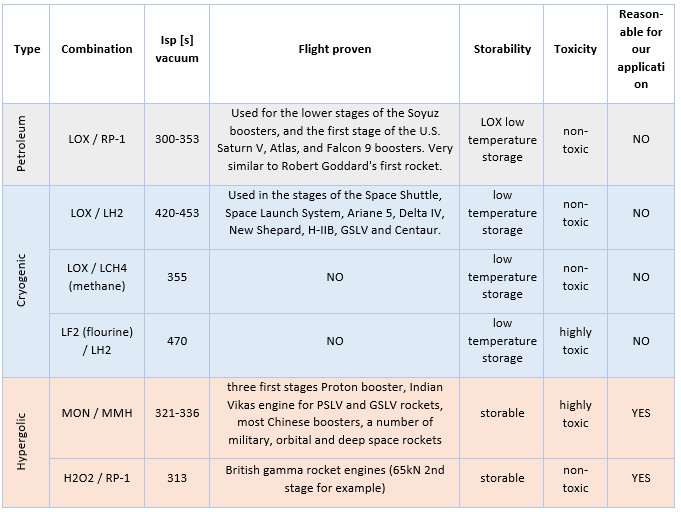
\includegraphics[width=\linewidth]{propcombination}
	
	\caption{Propellant combinations overview}\label{tab1}
\end{table}

\section{Detailed comparison between MON/MMH and H2O2/RP-1}
\qquad The hypergolic propellant combination MON/MMH and H2O2/RP-1 have been found reasonable for our mission and application. \autoref{tab2} shows a detailed comparison of the propellant combinations. Several characteristics were found to be minor and others were found to be major for our application. The major characteristics are the vacuum specific impulse, the tank volume ration, the combined density, the density specific impulse and the toxicity and storability (highlighted in yellow). \\

Both propellant combinations have a comparable specific impulse. Therefore no favor for either MON/MMH or H2O2/RP-1.\\

The tank volume ratio is better for MON/MMH because the ratio is nearly one to one, therefore both oxidizer and fuel tank could share the same tank design. This would significantly decrease the development costs since no second tank design and second qualification tank is necessary. Also the manufacturing costs would decreased due to more possibilities of batch production. Especially production costs of forged tank hemispheres are a huge cost driver and these would decrease due to non-recurring costs being distributed on a larger number of hemispheres.  Also the costs for jigs and tools would decrease. This favors MON/MMH.\\

The combined density for H2O2/RP-1 is slightly better than for MON/MMH. Nevertheless the combined density is not a significant value without taking the specific impulse into account. Calculating the density specific impulse, which is basically the specific impulse per mass, H2O2/RP-1 exceeds MON/MMH by 12\%. In this category H2O2/RP-1 is the winner because it can provide more specific impulse per mass.\\

Comparing toxicity of MON/MMH to H2O2/RP-1 it can be stated that MON/MMH is highly toxic and has to be handled with extreme care which increases the ground handling costs of this propellant combination. In contrast to that is the toxicity of H2O2/RP-1. This propellant combination is non-toxic and can be considered as “green” propellant. Nevertheless careful ground-handling is also necessary for this combination because it is prone to reaction with trace elements. H2O2/RP-1 succeeds in this category.\\

The last category is the storability. Since both propellant combinations are storable in liquid/liquid condition both propellants are suitable for the application.\\

Taking all criteria and results into account H2O2/RP-1 is the preferred propellant combination for our application. The main reasons are:
\begin{itemize}
	\item	comparable specific impulse to MON/MMH
	\item	better density specific impulse
	\item	non-toxic advantage for maintenance at refuel station
	\item	good on-ground handling
	\item	possibility of R\&D funds by ESA for green debris remover	
\end{itemize}

The main reason against MON/MMH is the toxicity.

\begin{table}
	\centering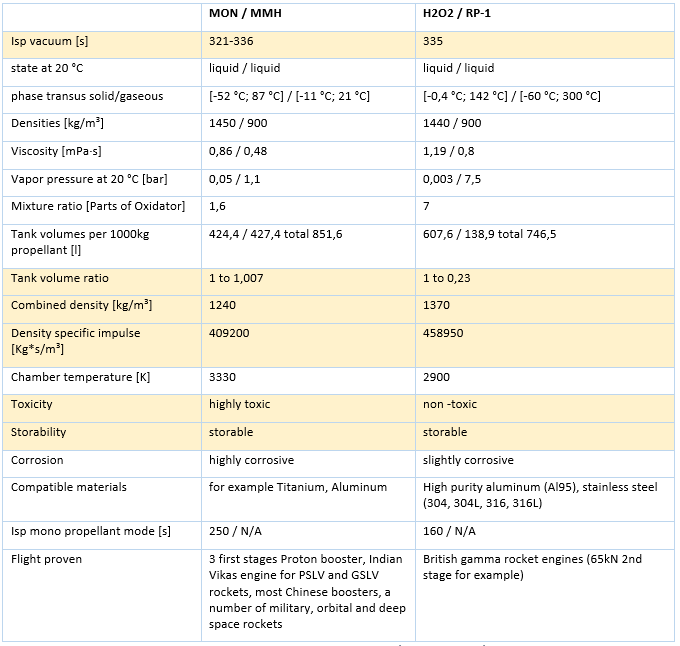
\includegraphics[width=\linewidth]{detailedcompprop}
	\caption{Detailed propellant comparison MON/MMH and H2O2/RP-1}\label{tab2}
\end{table}
\section{H2O2/RP-1 feasibility check}
\qquad Since H2O2/RP-1 is not a common propellant combination and not as frequently used space industry as MON/MHH a further feasibility study has to be performed:

\begin{itemize}
	\item	to de-risk the next development steps
	\item	to check whether the desired propellant combination is able to perform the required mission
\end{itemize}

In \ref{tab3} historical data of flight H2O2/RP-1 engines is analyzed. One of the engines “Gamma-2” was flown, the others were in development. The thrusts of all engines are comparable or higher than foreseen for our application and two engines also operate in comparable delta-v ranges. This leads to the conclusion that a H2O2/RP-1 engine is generally speaking feasible.

\begin{table}
	\centering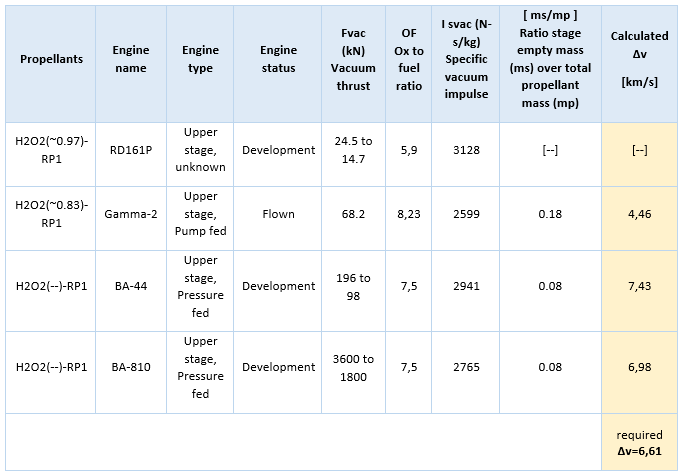
\includegraphics[width=\linewidth]{histflightprop}
	\caption{Historical data of flight H2O2/RP-1 engines}\label{tab3}
\end{table}
\section{Summary}

\qquad In summary H2O2/RP-1 is a viable non-toxic hypergolic propellant combination with a good density specific impulse. Additionally the propellant combination is supported by historical flight data. Therefore all further steps will be based on this combination.
\chapter{Vehicle design}
\chapter{Mass model and burning times}
\qquad \underline{By} : Julien
\section{Mass Budget - First Iteration}

\qquad Before actually going into our mass budget, we wanted to get a reference
idea for the propellant mass so that we would be sure to be able to
achieve our \(\Delta v\). In order to get this, we decided to find a
relation between the usable propellant mass and the mass of the rest as
a ratio. This is then fixed and will also allow us to know roughly how
much propellant we need depending on the dry mass. Let \(m_{UP}\) be the
mass of usable propellant. Moreover, we would be aiming for a total initial mass of roughly $20$ to $25t$ on our last iteration. This first iteration was done with another magnet design, presented in November which consisted in two large discs of $600\ kg$ each and have then been abandoned for the second iteration.


\subsection{Coefficients \& Masses after steps}

Considering that \(ISP = 295s\) and annotating
\(\frac{m_{UP_i}}{m_{total_i}} = K_i\) with \(i\) the burn number :

\begin{longtable}[]{@{}cccc@{}}
\toprule
Step & Required \(\Delta v\) in \(m/s\) & \(K_i\) & Mass after
step\tabularnewline
\midrule
\endhead
1 & 2802.4 & 0.620 & 0.38 \(m_{initial}\)\tabularnewline
2 & 1342.2 & 0.371 & 0.239\(m_{initial}\)\tabularnewline
3 & 522.9 & 0.165 & 0.200\(m_{initial}\)\tabularnewline
Satellite caught & NA & NA & 0.2\(m_{initial}\) + 3500\tabularnewline
4 & 1487.8 & 0.402 & 0.1196\(m_{initial}\) + 2093\tabularnewline
Satellite release & NA & NA & 0.1196\(m_{initial}\) -
1407\tabularnewline
5 & 5.3 & 0.002 & 0.1194\(m_{initial}\) - 1404.186\tabularnewline
6 & 72.4 & 0.0247 &\tabularnewline
\bottomrule
\end{longtable}


\subsection{Global equation between $m_{UP}$ and
	$m_{initial}$}

\begin{longtable}[]{@{}ccc@{}}
\toprule
Step & \(\frac{m_{UP}}{m_{initial}}\) & Bias due to
debris\tabularnewline
\midrule
\endhead
1 & 0.620 & 0\tabularnewline
2 & 0.141 & 0\tabularnewline
3 & 0.039 & 0\tabularnewline
4 & 0.0804 & 1407\tabularnewline
5 & 0.00024 & -2.814\tabularnewline
6 & 0.00295 & -36.68\tabularnewline
TOTAL & 0.88359 & +1369.506\tabularnewline
\bottomrule
\end{longtable}

We then get our general relation between the usable propellant mass and
the initial mass

\[m_{prop} = 0.88359 m_{init} + 1369.506\]

And as \(m_{initial} = m_{UP} + m_{rest}\) :

\[m_{prop} = \frac 1{0.11641}\bigg[0.88359 m_{rest} + 1369.506\bigg]\]

\(m_{rest}\) includes the dry mass and the propellant required for the
ACS.

\subsection{First iteration of mass budget}


\subsubsection{Sub systems}

\begin{longtable}[]{@{}cc@{}}
\toprule
Contributor & Mass in kg\tabularnewline
\midrule
\endhead
\underline{\textbf{EPS}} & -\tabularnewline
Fuel cells & 165.6727\tabularnewline
H2 for fuel cell (tank included) & 10\tabularnewline
Cables & 20\tabularnewline
GNC & 5\tabularnewline
Batteries & 61.3333\tabularnewline
Actuators (for flaps) & 10\tabularnewline
Servos & 1\tabularnewline
\underline{\textbf{On board computer}} & 5\tabularnewline
\underline{\textbf{Telecommunications}} & 10\tabularnewline
\underline{\textbf{Thermal control}} & 10\tabularnewline
\underline{\textbf{ACS/RCS}} & -\tabularnewline
Reaction wheels & 106\tabularnewline
ACS (without propellant) & 36.16\tabularnewline
\underline{\textbf{\emph{Total}}} & 440.166\tabularnewline
\bottomrule
\end{longtable}


\subsubsection{Payload}

\begin{longtable}[]{@{}cc@{}}
\toprule
Contributor & Mass in kg\tabularnewline
\midrule
\endhead
Magnet & 1200\tabularnewline
\bottomrule
\end{longtable}


\subsubsection{Structure}

\begin{longtable}[]{@{}cc@{}}
\toprule
Contributor & Mass in kg\tabularnewline
\midrule
\endhead
Hull & 509\tabularnewline
Wing & 54\tabularnewline
Engine & 60\tabularnewline
Engine frame & 51\tabularnewline
Connectors & 25\tabularnewline
Tanks & 350\tabularnewline
Heat shield & 472\tabularnewline
\underline{\textbf{\emph{Total}}} & 1521\tabularnewline
\bottomrule
\end{longtable}


\subsubsection{Others}

\begin{longtable}[]{@{}cc@{}}
\toprule
Contributor & Mass in kg\tabularnewline
\midrule
\endhead
Catalyzer & 10\tabularnewline
Lines & 25\tabularnewline
ACS including Propellant & 672\tabularnewline
Non usable propellant (Residuals, transient, etc.) & 200\tabularnewline
Helium (including tank) & 30\tabularnewline
\underline{\textbf{\emph{Total}}} & 937\tabularnewline
\bottomrule
\end{longtable}

We then get

\[m_{rest} = m_{Sub systems} + m_{Payload} + m_{Structure} + m_{Others} = 4098.166kg\]

Which, with the previously obtained equation :

\[m_{UP} = 42\ 870.926kg\\\]

As the mixture ratio is $MR = 7.07$ and $m_{UP} = m_{UF} + m_{UOP}$\\
\begin{align*}
m_{UsableFuel} &= \frac{m_{UP}}{1 + MR} = 5\ 312kg\\
m_{UsableOxidizer} &= MR \times m_{UsableFuel} =37\ 559kg
\end{align*}

\subsubsection{Results}
We can sum this first iteration up with the following table :

	\begin{table}[H]
\centering
	
\begin{tabular}[H]{|c|c|}
	\hline
	\cellcolor{gray!50}\textbf{Contributor} & \cellcolor{green!20}\textbf{Mass} (kg)\\
	\hline
	\textbf{Structure} & $1\ 521$\\
	\hline
	\textbf{Magnets} & $1\ 200$\\
	\hline
	\textbf{Sub Systems} & $440.166$\\
	\hline
	\textbf{Tank Pressurization} & $30$\\
	\hline
	\textbf{Engine} & $60$\\
	\hline
	\textbf{Catalyzer} & $10$\\
	\hline
	\textbf{Lines} & $25$\\
	\hline
	\cellcolor{gray!50}\textbf{Dry mass} & \cellcolor{green!20} $3\ 286.166$\\
	\hline
	\textbf{Non usable propellant} & $200$\\
	\hline
	\textbf{ACS/RCS Propellant} & $142. 12$\\
	\hline
	\textbf{Usable propellant} & $42\ 870.926$\\
	\cellcolor{red!50}\textbf{Total initial mass} & \cellcolor{red!50}$46\ 969.092$\\
	\hline 
\end{tabular}
\caption{Initial mass budget}
\end{table}

This first initial mass is way over what we are targeting and there are many parameters to be refined during the next iteration.
\newpage
\section{Mass Budget - Second iteration}
\qquad After refining multiple parameters and fixing others to get more accurate values, we went into the second iteration of our mass budget. Having our $I_{SP}$ changed also required another iteration in our calculation formula between the usable propellant mass the the rest of the mass.

\subsection{Coefficients \& Masses after steps}

Considering that \(ISP = 315s\) and annotating
\(\frac{m_{UP_i}}{m_{total_i}} = K_i\) with \(i\) the burn number :

\begin{longtable}[]{@{}cccc@{}}
\toprule
Step & Required \(\Delta v\) in \(m/s\) & \(K_i\) & Mass after
step\tabularnewline
\midrule
\endhead
1 & 2802.4 & 0.596 & 0.404 \(m_{initial}\)\tabularnewline
2 & 1342.2 & 0.352 & 0.261792\(m_{initial}\)\tabularnewline
3 & 522.9 & 0.156 & 0.221\(m_{initial}\)\tabularnewline
Satellite caught & NA & NA & 0.221\(m_{initial}\) + 3500\tabularnewline
4 & 1487.8 & 0.382 & 0.137\(m_{initial}\) + 2163\tabularnewline
Satellite release & NA & NA & 0.137\(m_{initial}\) -1337\tabularnewline
5 & 5.3 & 0.0017 & 0.1368\(m_{initial}\) - 1334.73\tabularnewline
6 & 72.4 & 0.023 &\tabularnewline
\bottomrule
\end{longtable}


\subsection{\texorpdfstring{Global equation between \(m_{UP}\) and
		\(m_{initial}\)}{Global equation between m\_\{UP\} and m\_\{initial\}}}
\begin{longtable}[]{@{}ccc@{}}
\toprule
Step & \(\frac{m_{UP}}{m_{initial}}\) & Bias due to
debris\tabularnewline
\midrule
\endhead
1 & 0.596 & 0\tabularnewline
2 & 0.142 & 0\tabularnewline
3 & 0.041 & 0\tabularnewline
4 & 0.084 & 1337\tabularnewline
5 & 0.0002 & -2.273\tabularnewline
6 & 0.0032 & -30.699\tabularnewline
TOTAL & 0.8664 & +1304.028\tabularnewline
\bottomrule
\end{longtable}



This time our equation between those two masses is given by 
\begin{equation}
m_{UsableProp} = \frac 1{0.1336}\bigg[0.8664 m_{rest} + 1304.028\bigg]
\end{equation}

\subsection{Second iteration of mass budget}

\qquad As our way of presenting our first iteration of the mass budget didn't seems clear enough to us, we decided to present it in another, more logical way :
\textbf{\underline{Structure}}
\begin{center}
\begin{tabular}[H]{|c|c|}
	\hline
	\cellcolor{gray!50}Contributor & \cellcolor{gray!50}Mass (kg)\\
	\hline
	Hull & $192$\\
	\hline
	Tanks (including non usable propellant) & $700$\\
	\hline
	Wings & $136$\\
	\hline
	Lines & $60$\\
	\hline
	Connectors & $16$\\
	\hline
	$H_2$ tank & $12$\\
	\hline
	\cellcolor{green!30}\textbf{Structure} & \textbf{$1\ 116$}\\
	\hline
\end{tabular}
\end{center}

\textbf{\underline{Electrical related contributors}}
\begin{center}
\begin{tabular}[H]{|c|c|}
	\hline
	\cellcolor{gray!50}Contributor & \cellcolor{gray!50}Mass (kg)\\
	\hline
	Batteries & $241$\\
	\hline
	Fuel cells & $202$\\
	\hline
	On Board Computer & $5$\\
	\hline
	Cables & $20$\\
	\hline
	$H_2$ for fuel cells & $5$\\
	\hline
	Wing actuators & $10$\\
	\hline
	Telecommunications & $10$\\
	\hline
	GNC & $5$\\
	\hline
	Thermal Control & $10$\\
	\hline
	Magnets (Payload) & $25.65$\\
	\hline
	\cellcolor{green!30}\textbf{Electrical related contributors} & \textbf{$533.65$}\\
	\hline
\end{tabular}
\end{center}

\textbf{\underline{ACS and RCS}}
\begin{center}
\begin{tabular}[H]{|c|c|}
	\hline
	\cellcolor{gray!50}Contributor & \cellcolor{gray!50}Mass (kg)\\
	\hline
	Thrusters & $36$\\
	\hline
	$H_2O_2$ & $90$\\
	\hline
	Reaction wheels & $106$\\
	\hline
	\cellcolor{green!30}\textbf{ACS \& RCS} & \textbf{$232$}\\
	\hline
\end{tabular}
\end{center}

\textbf{\underline{Propulsion}}
\begin{center}
\begin{tabular}[H]{|c|c|}
	\hline
	\cellcolor{gray!50}Contributor & \cellcolor{gray!50}Mass (kg)\\
	\hline
	Engine & $93$\\
	\hline
	Turbopumps & $25$\\
	\hline
	Pressurization ($He$) & $1.3$\\
	\hline
	Catalyzer & $30$\\
	\hline
	\cellcolor{green!30}\textbf{Propulsion} & \textbf{$149.3$}\\
	\hline
\end{tabular}
\end{center}

With those tables, we can deduce $m_{rest}$ :
\begin{align}
m_{rest} &= m_{Structure} + m_{Elec} + m_{ACS\&RCS} + m_{Propulsion}\\
m_{rest} &= 2\ 030.95kg
\end{align}
Thus,
\begin{align}
m_{UsableProp} &= \frac 1{0.1336}\bigg[0.8664 m_{rest} + 1304.028\bigg]\\
m_{UsableProp} &= 22\ 931kg\\
m_{Fuel} &= \frac{m_{UsableProp}}{MR+1}\\
m_{Fuel} &= 2841.6kg\\
m_{Ox} &= m_{UsableProp} - m_{Fuel}\\
m_{Ox} &= 20\ 089.89kg\\
m_0 &= 24\ 962.41kg
\end{align}



In this second iteration with a better \(I_{sp}\) and refined values for all of the contributors, we have a large improvement as our initial mass decreased drastically.
\newpage
\section{Frozen information}[H]
After our second iteration of the mass budget, we decided to make a list of the fixed values that we will work around in our further design.
\subsection{Frozen points}
\begin{itemize}
\item We will do $20$ aerobrakes
\item We will have a separate tank design
\item $H_2O_2$ will be pressurized by its decomposition
\item The decomposition control will be managed by rotation of the spacecraft
\item ACS/RCS Layout similar to the Space Shuttle
\item $H_2O_2$ catalyzers separate
\item $H_2O_2/O_2$ separation via thermodynamic properties
\item $H_2/O_2$ will be used in fuel cells to produce energy
\end{itemize}
\begin{table}
\centering
\begin{tabular}[H]{|c|c|c|}
	\hline
	\cellcolor{gray!50}Data & \cellcolor{gray!50}Value & \cellcolor{gray!50}Unit\\
	\hline
	Empty raw mass & $2\ 031$ & kg\\
	\hline
	Usable propellant & $22\ 931$ &kg\\
	\hline
	\cellcolor{green!50}Total mass & \cellcolor{green!50}$24\ 962$ & \cellcolor{green!50}kg\\
	\hline
	Flowrate & $10$ & kg/s\\
	\hline
	Rocket diameter & $2$ & $m$\\
	\hline
	$I_{sp_{vacuum}}$ & $335$ & s\\
	\hline
	Thrust $F=\dot m I_{sp} g_0$ & $32 863.5$ &N\\
	\hline
	Mixture Ratio & $7.07$ & -\\
	\hline
	Wall thickness & $TBA$ & m\\
	\hline
	$H_2O_2$ internal pressure & $1.35$ & bar\\
	\hline
\end{tabular}
\caption{Frozen information}
\end{table}

\newpage
\section{Mass Budget - Final iteration}
As the fixed $I_{sp}$ has been refined as well as other parameters, we went into our final iteration of the mass budget with the same process as the two previous ones.
\subsection{Coefficients \& Masses after steps}

Considering that \(ISP = 335s\) and annotating
\(\frac{m_{UP_i}}{m_{total_i}} = K_i\) with \(i\) the burn number :

\begin{longtable}[]{@{}cccc@{}}
\toprule
Step & Required \(\Delta v\) in \(m/s\) & \(K_i\) & Mass after
step\tabularnewline
\midrule
\endhead
1 & 2802.4 & 0.574 & 0.426 \(m_{initial}\)\tabularnewline
2 & 1342.2 & 0.335 & 0.283\(m_{initial}\)\tabularnewline
3 & 522.9 & 0.148 & 0.241\(m_{initial}\)\tabularnewline
Satellite caught & NA & NA & 0.241\(m_{initial}\) + 3500\tabularnewline
4 & 1487.8 & 0.364 & 0.153\(m_{initial}\) + 2226\tabularnewline
Satellite release & NA & NA & 0.153\(m_{initial}\) -1274\tabularnewline
5 & 5.3 & 0.0016 & 0.1528\(m_{initial}\) - 1271.96\tabularnewline
6 & 72.4 & 0.0218 & (0.1495$m_{initial}$ - 1244.23)\tabularnewline
\bottomrule
\caption{Coefficients and masses after steps}
\end{longtable}


\subsection{\texorpdfstring{Global equation between \(m_{UP}\) and
		\(m_{initial}\)}{Global equation between m\_\{UP\} and m\_\{initial\}}}



\begin{longtable}[]{@{}ccc@{}}
\toprule
Step & \(\frac{m_{UP}}{m_{initial}}\) & Bias due to
debris\tabularnewline
\midrule
\endhead
1 & 0.574 & 0\tabularnewline
2 & 0.143 & 0\tabularnewline
3 & 0.042 & 0\tabularnewline
4 & 0.088 & 1274\tabularnewline
5 & 0.0002 & -2.038\tabularnewline
6 & 0.0033 & -27.73\tabularnewline
TOTAL & 0.8505 & +1244.232\tabularnewline
\bottomrule
\end{longtable}
Thus,
$$
m_{UsablePropellant} = \frac 1{0.1495}[0.8505m_{rest}+1244.232]
$$
\subsection{Detailed contributors}
\subsubsection{Structure}
\begin{table}

\begin{center}
\begin{tabular}[H]{|c|c|}
	\hline
	\cellcolor{gray!50}Contributor & \cellcolor{gray!50}Mass (kg)\\
	\hline
	Hull & $192$\\
	\hline
	Tanks & $700$\\
	\hline
	Wings & $136$\\
	\hline
	Lines & $70$\\
	\hline
	Connectors & $16$\\
	\hline
	Brackets & $35$\\
	\hline
	$H_2$ Tanks & $12$\\
	\hline
	\cellcolor{green!30}\textbf{Structure} & \textbf{$1161$}\\
	\hline
\end{tabular}
\end{center}
\label{Mass budget - Structure}	
\end{table}
\subsubsection{Electrical systems}
\begin{table}
	
\begin{center}
\begin{tabular}[H]{|c|c|}
	\hline
	\cellcolor{gray!50}Contributor & \cellcolor{gray!50}Mass (kg)\\
	\hline
	Batteries & $388.66$\\
	\hline
	Fuel cell & $202$\\
	\hline
	OBC & $10$\\
	\hline
	Cables & $57$\\
	\hline
	$H_2$ for fuel cells & $5$\\
	\hline
	Wing actuators & $10$\\
	\hline
	Data transmission & $10$\\
	\hline
	GNC & $10$\\
	\hline
	Thermal control & $20$\\
	\hline
	Magnets & $25.65$\\
	\hline
	\cellcolor{green!30}\textbf{Electrical systems} & \textbf{$738.31$}\\
	\hline
\end{tabular}
\end{center}
\caption{Mass budget - Electrical systems}
\end{table}
The mass of the batteries is given by $m_{Bat} = \frac{E_{pumps} + E_{magnet}}{ED_{Lithium}}$ with a considered energy density of $100Wh/kg$
\subsubsection{Attitude control}
\begin{table}
	
\begin{center}
\begin{tabular}[H]{|c|c|}
	\hline
	\cellcolor{gray!50}Contributor & \cellcolor{gray!50}Mass (kg)\\
	\hline
	Thrusters & $36$\\
	\hline
	$H_2O_2$ for the ACS & $90$\\
	\hline
	
	Reaction wheels & $106$\\
	\hline
	\cellcolor{green!30}\textbf{Attitude control} & \textbf{$232$}\\
	\hline
\end{tabular}
\end{center}
\caption{Mass Budget - Attitude Control}
\end{table}
\subsubsection{Propulsion}
\begin{table}
	
\begin{center}
\begin{tabular}[H]{|c|c|}
	\hline
	\cellcolor{gray!50}Contributor & \cellcolor{gray!50}Mass (kg)\\
	\hline
	Engine & $93$\\
	\hline
	Turbopumps + Electric motors & $170$\\
	\hline
	$He$ for pressurization & $1.3$\\
	\hline
	Catalyzer & $40.86$\\
	\hline
	\cellcolor{green!30}\textbf{Propulsion} & \textbf{$305.16$}\\
	\hline
\end{tabular}
\end{center}
\caption{Mass Budget - Propulsion}

\end{table}
\subsection{Final mass budget}

\begin{table}[H]
	\centering
\begin{tabular}[H]{|c|c|}
	\hline
	\cellcolor{gray!50}Contributor & \cellcolor{gray!50}Mass (kg)\\
	\hline
	Structure & $1161$\\
	\hline
	Electrical systems & $738.31$\\
	\hline
	Attitude control & $232$\\
	\hline
	Heat shield & $360$\\
	\hline
	Propulsion & $305.16$\\
	\hline
	\cellcolor{green!30}\textbf{$m_{rest}$} & \textbf{$2796.5$}\\
	\hline
	\cellcolor{green!30}\textbf{$m_{UP}$} with a $5\%$ performance window & \textbf{$25\ 505$}\\
	\hline
	\cellcolor{green!30}\textbf{$m_{Fuel}$}  & \textbf{$3160. 5$}\\
	\hline
	\cellcolor{green!30}\textbf{$m_{Ox}$}  & \textbf{$22\ 345$}\\
	\hline
	\cellcolor{red!30}\textbf{Initial wet mass}  & \textbf{$28\ 302$}\\
	\hline
\end{tabular}
\caption{Final mass budget}
\end{table}
\section{Burn times}
\qquad From the tables of $\Delta v$ and related mass-ratios (from the Tsiolkovsky Equation), we can get the burn times as, for each step, the burn time is defined by : 
\begin{equation}
	t_{burn} = \frac{\Delta m_{step}}{\dot{m}}
\end{equation}
With $\dot{m}$ being the general mass flow of $10$ kg/s. We separate our first step into two different burns. 
\begin{equation}
	\Delta m_j  = m_{j-1}
\end{equation}
\begin{table}
	\centering
	\begin{tabular}{|c|c|}
		\hline
		Step & Mass after step (kg)\\
		\hline
		1 & 12 056.652\\
		\hline
		2 & 8 009.466\\
		\hline
		3 & 6 820.782\\
		\hline
		Catch & 9 754.742\\
		\hline
		4 & 6 556.206\\
		\hline
		Release & 3 056.206\\
		\hline
		5 & 3 052.586\\
		\hline
		6 & 2 986.039\\
		\hline
	\end{tabular}
	\caption{Masses after step} \label{tabmass}
\end{table}
\begin{table}[H]
	\centering
	\begin{tabular}{|c|c|c|c|}
		\hline
		Step & $\Delta v_{step}(m/s)$ &  $\Delta m_{step} (kg)$ & $t_{burn} (s)$\\
		\hline
		1 & 2802.4 &  16 245.35 & 1 624.535 (separate into two burns)\\
		\hline
		2 & 1342.2 & 4 047.19 & 404.719\\
		\hline
		3 & 522.9 & 1 188.684 & 118.868\\
		\hline
		4 & 1487.8 & 3 198.536 & 319.854\\
		\hline
		5 & 5.3 & 3.62 & 0.362\\
		\hline
		6 & 72.4 & 66.817 & 6.682\\
		\hline
		TOTAL & 6 233 &  & 2 475.02\\
		\hline
	\end{tabular}
\end{table}
\chapter{Propulsion system}
\section{Engine cycle}
\qquad The spacecraft uses electrically-driven turbo pumps to feed the oxidizer as well as the fuel to the engine. The propellant and oxidizer are each driven out of their tanks at low pressure, where after a turbo pump in each propellant line strain raises their pressures. As the oxidizer strain has a higher mass flow rate and faces a large pressure drop in the catalyzer, the respective pump is also more powerful as a result. The turbo pumps are driven electrically by electric motors which use large batteries for their power intake. These batteries offer enough charge for one maximum burn time of 900 seconds, after which they are re-powered by a fuel cell which runs on hydrogen and the hydrogen peroxide decomposition product oxygen. This will be explained further in \autoref{sec:10-3}. In order to demonstrate how exactly the engine cycle is made up, a flow schematic is shown in the following. Firstly, the pressurization system is shown in \autoref{fig1}.
\begin{figure}[H]
	\centering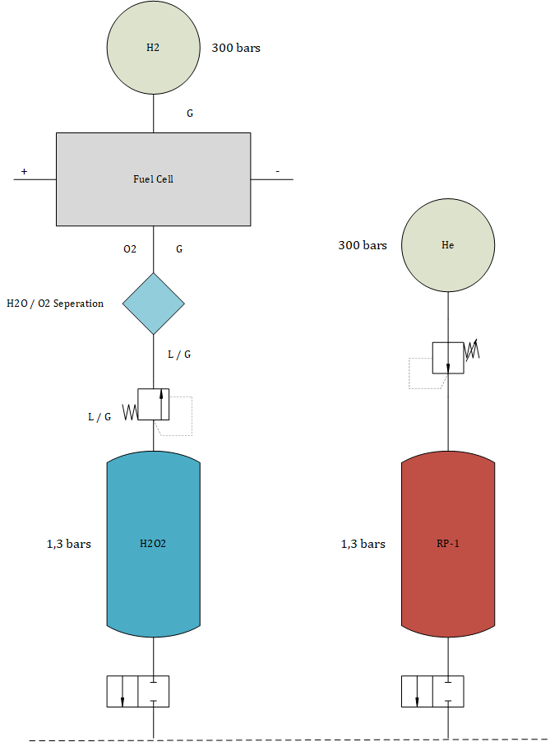
\includegraphics[width=0.5\linewidth]{pressurizationsystem}
	\caption{Flow Schematic - Pressurization system}\label{fig1}
\end{figure}

As the figure shows, only the RP-1 tank is pressurized by pressurization gas, using a $300$ bars helium tank. The hydrogen peroxide has certain decomposition characteristics which enable it to self-pressurize due to the rising pressure upon vaporization. The critical point of hydrogen peroxide is at around $150$ degrees Celsius and $1.5$ bars, meaning that if the thermal control is sufficiently reliable, a tank pressure of around $1.3$ bars can be maintained by self-pressurization. The control system and more details will be explained in \autoref{sec:10-3}. The $300$ bars H2 Tank that can be seen in the pressurization system flow schematic is therefore not a pressurization tank, but a tank for the sole purpose of running the fuel cell in combination with the oxygen which is separated from water, which is the second decomposition product of hydrogen peroxide. The separation works by simply condensing the water and allowing the gaseous oxygen to pass through a filter. Both the RP-1 tank and the H2O2 tank have a main valve after their outlets, which are visible in \autoref{fig1}. The remaining feeding system is shown in the second part of the flow schematic, depicted in \autoref{fig2}.

\begin{figure}[H]
	\centering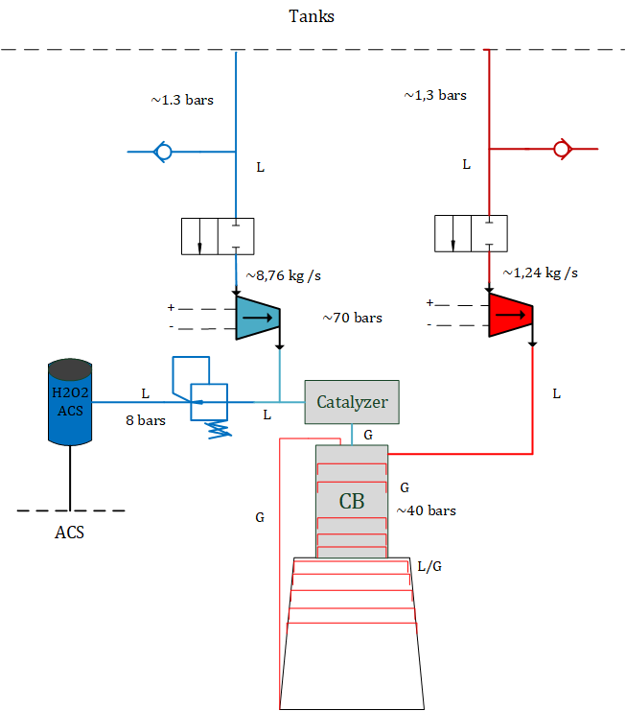
\includegraphics[width=0.7\linewidth]{flowenginesection}
	\caption{Flow Schematic - Engine section}\label{fig2}
\end{figure}
The fueling ports for RP-1 as well as hydrogen peroxide extend to the left- and right-hand-side of the top of the figure. Check valves are situated at these points to only allow propellant flowing in. A second main valve for both propellants is installed just before the turbopumps, which are closed during refueling. While the RP-1 is then funneled through cooling channels in the regenerative cooling system, the oxidizer runs into a catalyzer, where a rapid decomposition reaction splits the hydrogen peroxide into its reactive products for combustion. A second oxidizer strain is guided towards a pressure regulation valve, behind which it continues into a buffer tank of hydrogen peroxide for monopropellant use in the ACS. The catalyzers for ACS thrusters are located in close proximity to their respective combustion chambers. The ACS is not depicted as a flow schematic.

\section{RCS / ACS}

In the previous section we mention that we are going to use hydrogen peroxide as a monopropellant for our Reaction Control System. Indeed, hydrogen peroxide can be used as a quite good RCS propellant. \\

At the moment, the biggest part of the monopropellant thruster using $H_2O_2$ are test bench engine. This is because of the difficulty to characterize the engine and its parameters. \\

Hydrogen peroxide is usable as a monopropellant because of its natural decomposition. As we are going to see on the Catalyzer part further on the report $H_2O_2$ can be decomposed in $H_2$ and $H_2O$. That's this decomposition we are going to use inside our thruster. \\
When hydrogen peroxide goes through a catalyser it decomposes and generates a great amount of heat, up to $1000K$. This two factors create steam at a very high temperature and pressure; it's this steam that creates our thrust.\\

Before designing the engine and its characteristics we need to choose the positioning of the thrusters. In order to do that, we based our design on the American Space Shuttle which use cluster of small thrusters all around the spacecraft to allow a good maneuverability.  

\begin{figure}[H]
    \centering
    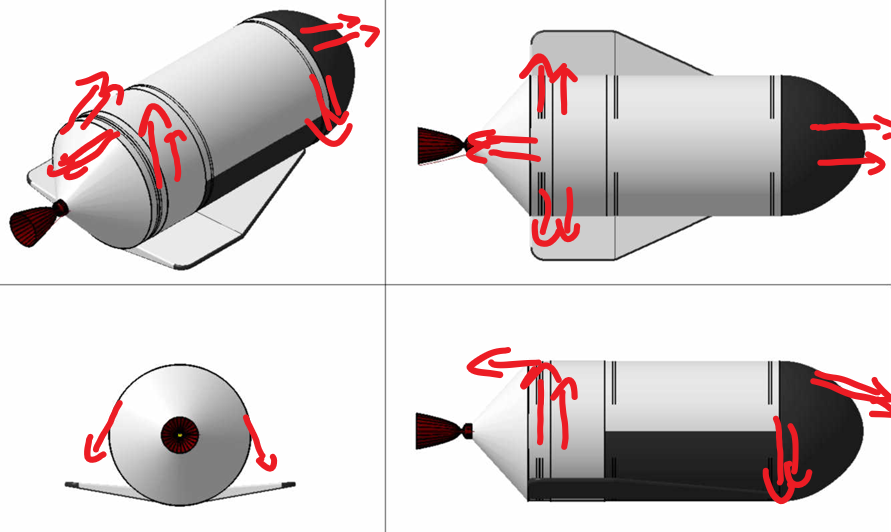
\includegraphics[width=\linewidth]{shiprcs}
    \caption{RCS thruster repartition}
\end{figure}

We are going to use 6 different clusters spread over the craft, each cluster is composed of 2 thrusters for a total of 12. This disposition allow to manipulate every axis. \\

Now we need to compute the characteristic of the thruster, to do so we used RPA (a NASA software to compute the parameters of a thruster based on the propellant and several other characteristics) and some papers of recent studies about hydrogen peroxide thruster. \\

We assumed a chamber pressure of $10bars$ and a thrust of $100N$, then we use RPA to get the other parameters.

\begin{itemize}
    \item Combustion temperature: $1223K$
    \vspace{-0.4cm}
    \item Ejection temperature: $424K$
    \vspace{-0.4cm}
    \item Ejection pressure : $0.094bars$
    \vspace{-0.4cm}
    \item $\gamma = 1.335$
    \vspace{-0.4cm}
    \item $R = 368.6$
    \vspace{-0.4cm}
    \item $ISP = 140s$
\end{itemize}

With these parameters we can then compute every other parameters we want for the thruster and especially the mass flow rate which is necessary to have a correct mass budget. 

$$c^* = \sqrt{\frac{R T_c}{\gamma}}\times \frac{\gamma + 1}{2}^{\frac{\gamma + 1}{2(\gamma - 1)}}$$

Throat characteristics:
$$T_t = T_c \left(\frac{2}{\gamma + 1}\right) \hspace{20pt}
P_t = P_c \left(\frac{2}{\gamma + 1}\right)^{\frac{\gamma}{\gamma - 1}} \hspace{20pt}
\rho = \frac{P_t}{R T_t} \hspace{20pt}   u_t = \sqrt{\gamma R T_t}$$

Exhaust characteristics:
$$M_e = \sqrt{\frac{2}{\gamma - 1}\left[\left(\frac{P_c}{P_e}\right)^\frac{\gamma - 1 }{\gamma} - 1 \right]} \hspace{20pt} T_e = \frac{T_c}{1 + \frac{\gamma - 1}{2}M_e^2}  \hspace{20pt} \rho_e = \frac{P_e}{R T_e}$$

\clearpage

Thus we can compute the area ratio and the thrust coefficient:

$$\frac{A_e}{A_t}= \frac{1}{M_e}\left[\frac{2}{\gamma + 1}\left(1 + \frac{\gamma - 1}{2} M_e^2 \right)\right]^{\frac{\gamma + 1}{2(\gamma - 1)}}$$

$$ C_F = \gamma \sqrt{\left(\frac{2}{\gamma + 1}\right)^{\frac{\gamma + 1}{\gamma - 1}}\frac{2}{\gamma - 1} \left[ 1 - \left(\frac{P_e}{P_c}\right)^{\frac{\gamma - 1}{\gamma}}\right]} + \frac{P_e - P_a}{P_c}\frac{A_e}{A_t} $$ 

\vspace{1cm}

Finally we can compute the exhaust velocity, throat area and the mass flow: 

$$c = C_F c^* \hspace{20pt} A_t = \frac{F}{C_F P_c} \hspace{20pt} \dot m = \frac{P_c A_t}{c^*}$$

From our assumptions and the results of RPA we finally have:

\begin{itemize}
    \item Exhaust velocity: $c=617.38m/s$
    \vspace{-0.4cm}
    \item Mass flow rate: $\dot m = 0.105 kg/s$
\end{itemize}

The most important value for us is the mass flow rate as it allows us to compute the propellant mas needed to perform our maneuvers. \\

In addition of the thrusters we also need another system which is the Reaction Wheels. This systems which is separated in 3 different wheel, one for each axis, and allow to rotate the entire craft on the 3 axis with the the reaction motion applied by the rotation of the wheel.
\clearpage

\section{Multi-usage of hydrogen peroxide}
\label{sec:10-3}

\section{Propellant tanks}
The vehicle must use propellant tanks in order to carry the oxidizer and fuel, in this case H2O2 and RP-1, during the mission. The required total useable propellant was already found in the final mass budget calculation. 
This chapter describes the tank design beginning with the requirements and tank specification, afterwards the analysis of compatible materials following by the design including different options, expulsion principle, stresses, MAIT and final design. The Liner tanks are also addressed in the last part of this chapter.\\

\subsection{Requirements and specification}
Several parameters have to be set in prior to the propellant tank design in order to ensure that all top level vehicle and propulsion system requirements are met. Additionally it must be ensured that the propellant tank assemblies sustain launch and flight loads during all phases of the mission.
\subsubsection{Propellant Tank masses and volumes}

\autoref{tab:propmass} shows the calculated values of the final propellant mass and final volumes of both oxidizer and fuel. The basis of this calculation is the final mass budget that provided the useable propellant masses. Starting at this value and calculating 1\% additional propellant for ignition, 2\% for shutdown, 2\% performance reserve and 2\% residuals, the masses add up to 24t for H2O2 and 3.4t for RP-1. H2O2 needs a greater ullage volume than RP-1 due to the decomposition, with 20\% ullage a total tank volume of $\geq$ 18.62 m$^3$ is necessary. For RP-1 a total tank volume of  $\geq3.99$ m$^3$ needs to be accomplished.
\begin{table}[H]
    \centering
    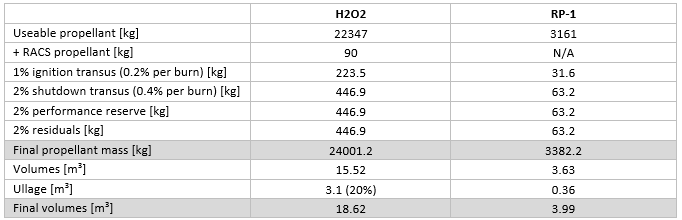
\includegraphics[width = \linewidth]{propmassvol}
    \caption{Propellant masses and volumes}
    \label{tab:propmass}
\end{table}{}
\subsubsection{Driving requirements}
The driving requirements for the oxidizer propellant tank assembly (PTA) are summarized in \autoref{tab:PTAreq}. MDP is taken according to \autoref{chap:2}
\begin{table}[H]
    \centering
    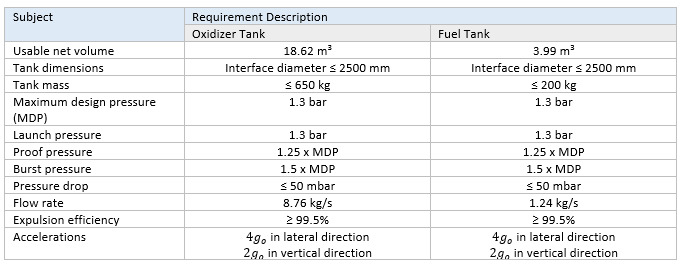
\includegraphics[width = \linewidth]{ptareq}
    \caption{PTA driving requirements}
    \label{tab:PTAreq}
\end{table}{}
\subsubsection{Pressure loads}
The ECSS requires a safety factor of 1.25 on proof pressure and 1.5 on burst pressure according to \autoref{chap:2}. Therefore the pressure levels including safety factors are listed in \autoref{tab:ptapress}.
\begin{table}[H]
	\centering
	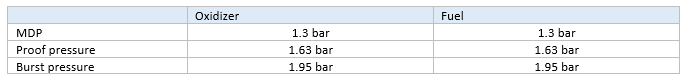
\includegraphics[width = \linewidth]{ptapress}
	\caption{PTA pressure loads}
	\label{tab:ptapress}
\end{table}{}
The number of pressure cycles after delivery is shown in \autoref{tab:ptacycle}. This number of pressure cycles applies for both the oxidizer and fuel tank.
\begin{table}[H]
	\centering
	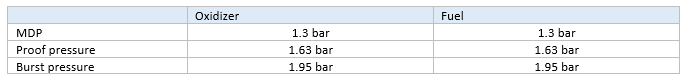
\includegraphics[width = 0.6\linewidth]{ptapress}
	\caption{PTA pressure cycles}
	\label{tab:ptacycle}
\end{table}{}
\pagebreak
\subsection{Materials}
The intended materials for the propellant tanks are listed in \autoref{tab:tankmat}. For the fuel tank and liner tanks a common titanium alloy can be used with high strength and good ductility. The titanium alloy shall be heat treated to .7 status (solution treated and aged) in order to achieve the below mentioned material characteristics and to stress relieve. The liner tanks can also be winded or wrapped with CFK in order to be further strengthened and to reduce the wall thickness of the titanium.\\

The oxidizer tank shall be manufactured of aluminum 5254 which is long term compatible and corrosion resistant against H2O2. Unfortunately the aluminum alloy shows a low strength which has to be taken into account in the mechanical calculations. A higher strength option of this alloy is currently in development acc. to NASA paper.
\begin{table}[H]
	\centering
	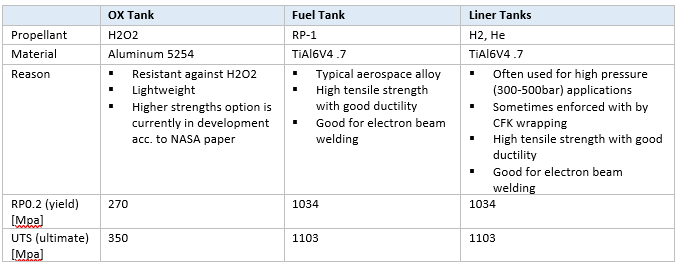
\includegraphics[width = \linewidth]{tankmat}
	\caption{Propellant tank materials}
	\label{tab:tankmat}
\end{table}{}
\pagebreak
\subsection{Concepts and options}
During the process of finding the optimum propellant tank concept for the GREDER vehicle, our mission and application, several possible design option have been taken into account. \autoref{fig:tankdesign} shows the three most promising options.\\

The first option is an integrated concept with the fuel tank placed within the oxidizer tank. Integrated designs are in theory the most lightweight design option for propellant tanks because the basic idea is to reduce the wall thickness of the inner tank due to theoretically no pressure delta between fuel and oxidizer tank pressure. The downside of this option is the manufacturing. Also the use of spacecraft volume is quite attractive with this design. Manufacturing of one tank inside of another tank and then welding it is a tough task. Additionally the fuel tank also needs to be compatible with both propellants because it is in contact with the oxidizer from the outside and the fuel from the inside. Therefore option 1 is not suitable for our application due to manufacturing complexity, material compatibility and our MDP of 1.3 bar is way too low to justify the advantage of wall thickness reduction.\\

The second option is also an integrated option but this time with two separate tanks. This slightly increases the spacecraft volume but is still more spacecraft volume efficient than option 3. This option, especially the special shape of the oxidizer tank, is a complex geometry and therefore also complex to manufacture. The fuel tank manufacturing is simpler than in the first option due to the half sphere hemispheres and gimbal mounting. During first attempts of a detailed design of that option it was found that the vehicle diameter increased over the boundary requirement. For this reason and also due to the complex manufacturing and design this option was found to not be the most efficient design for our application.\\

The third option is a rather simple “two-tanks-on-top-of-each-other” design. The main advantage is here the simple design and manufacturing and assembly of all parts, the possibility of load carrying structure of the outer tank walls as well as good options for tank expulsion principles. This design was found to be the optimum for our application and is therefore the baseline for all further calculations and detailed design.

\begin{figure}[H]
	\centering
	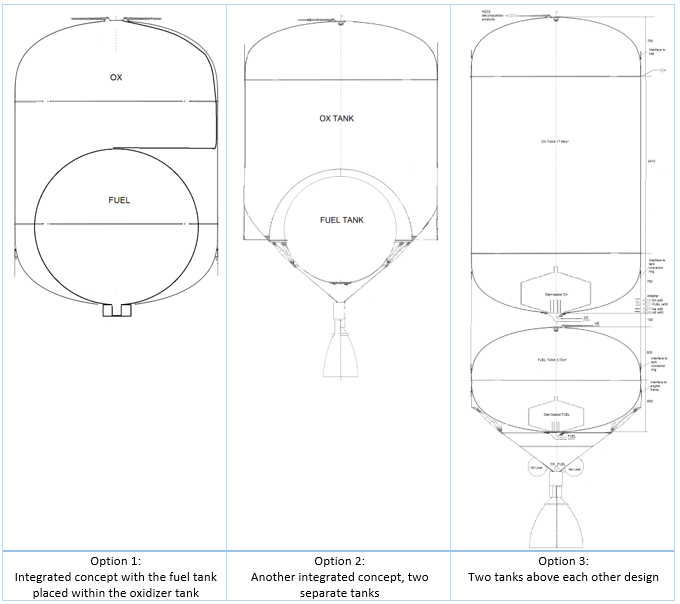
\includegraphics[width=\linewidth]{tankdesignoption}
	\caption{Different propellant tank design options}\label{fig:tankdesign}
\end{figure}
\section{Catalyzer}
Besides the advantages of $H_2O_2$ there is one major drawback that we have to take into account. This drawback is that $H_2O_2$ needs to be decomposed in $H_2$ and $H_2O$ in order to react with RP-1. 

\begin{figure}[H]
	\centering
	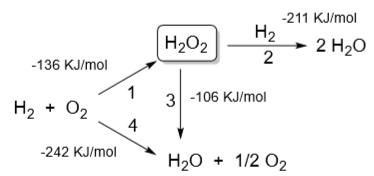
\includegraphics{H2O2}
	\caption{$H_2O_2$ chemical decomposition process}
\end{figure}

This decomposition is natural but at a low rate whereas we need a very high decomposition rate in order to feed the combustion chamber and sustain a proper flame. This decomposition is an exothermic decomposition. That's why we need a catalyser. \\

This catalyser needs to be placed between the turbo pump and the injectors. It allows to decompose the $H_2O_2$ at the last time. \\

The way a catalyser works is pretty simple; the $H_2O_2$ goes through a catalyst bed of silver pellets, reacts and generates heat. 
Why silver ? We chose silver because is the mostly used catalyser for $H_2O_2$. However, a lot of other different material exists, like Platinum, Manganese or even Gold but these materials are rarely used due to their cost and also the fact that they need to be made in complex alloy in order to optimize the reaction. 

\begin{figure}[H]
	\centering
	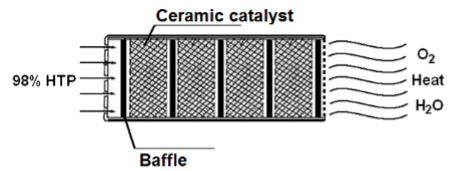
\includegraphics{catalyst}
	\caption{Example of catalyst bed}
\end{figure}

The figure above shows basically how a catalyser works. To have an idea of the shape of ours we just have to swap the ceramic catalyst by silver catalyst. So, it will be a steel cylinder filled with small spherical silver pellet separated by some baffles (silver grid mesh). \\

An important characteristic of the catalyser is the pressure drop it creates. This pressure drop influences the whole feeding system, the turbo pump sizing and even the injector design. that's why we need to characterize the pressure drop created by the catalyser. In order to do so, we are going to use the Ergun equation for packed bed reactor:

$$
\frac{\Delta p}{L} = 151.2 \frac{\mu}{d^2}\frac{(1-\epsilon)^2}{\epsilon^2}u + 1.8 \frac{\rho}{d}\frac{1- \epsilon}{\epsilon^3}u^2
$$

With $\mu$ the dynamic viscosity, $\epsilon$ the porosity, $d$ the pellet diameter, $\rho$ the density, $L$ the length of the bed and $u$ the velocity. \\

In this equation we need some important component such as $\epsilon$. The porosity is complicated to compute and need to be model. According to a recent research we determined a porosity of $0.3802$ with a pellet diameter of 5mm.

\begin{figure}[H]
	\centering
	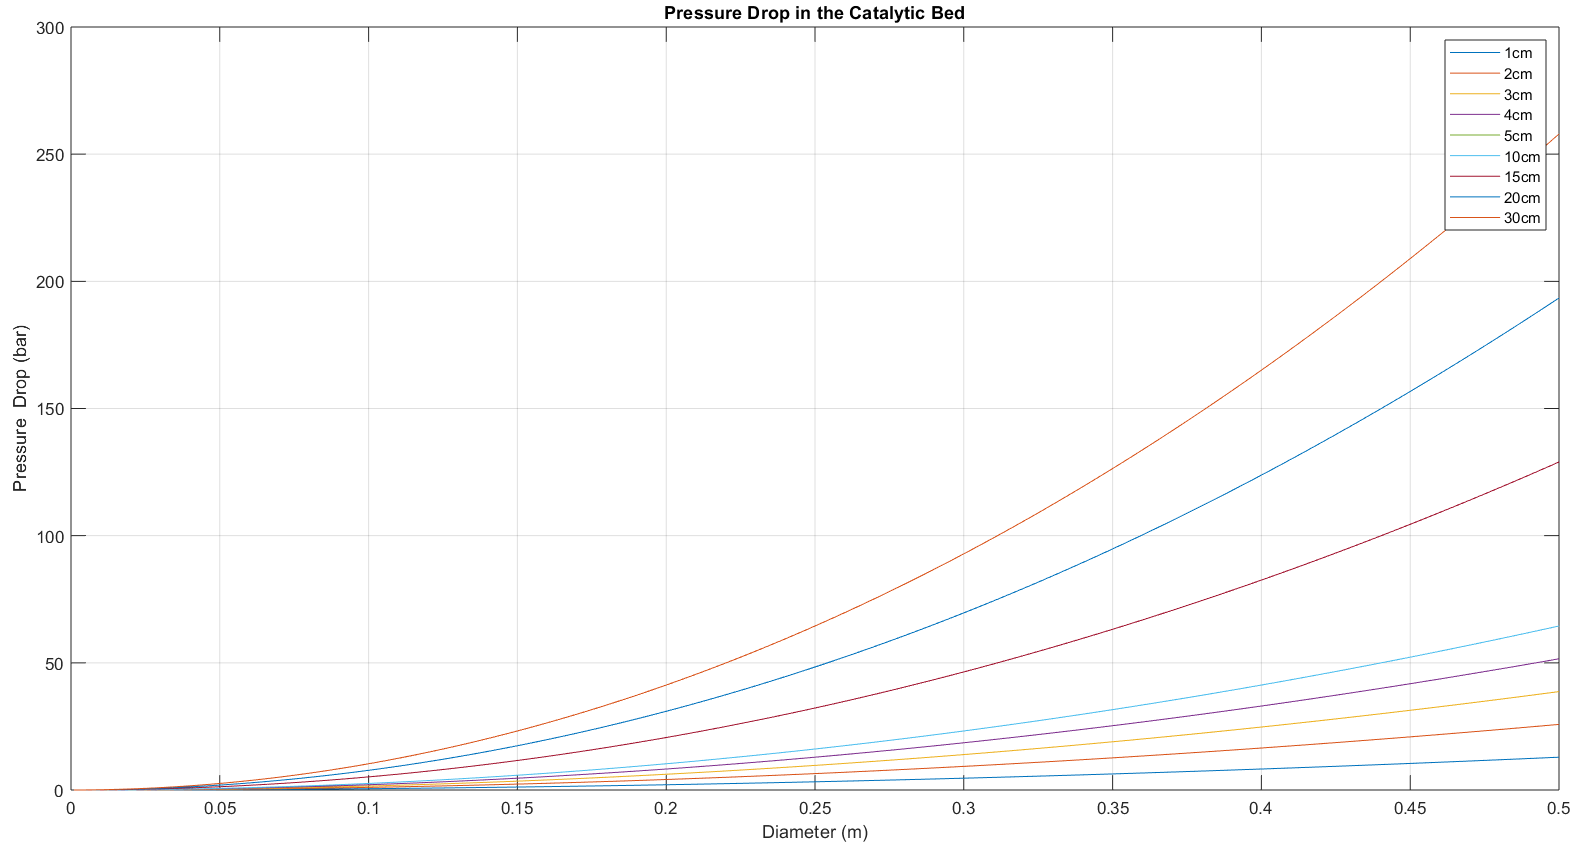
\includegraphics[width=\linewidth]{pressuredrop}
	\caption{Pressure drop depending on the size of the catalyst bed}
\end{figure}

We see on the graph that the pressure drop rise quickly with the size of the bed. So we need to limit the size of our catalyser in order to not oversize the turbo pump. To do so, we chose to limit our pressure drop to around 30 bars. Finally we obtain a cylinder of 20 cm of diameter and 20 cm of length. \\

This geometry allows the catalyser to provide a sufficient decomposition rate, a "contained" pressure drop and size. It also generates a great heat as high as $1000K$ at the exit of the catalyst bed. 

\section{Injectors}

To design our injectors we made some research and went through the literature about injector for hypergolic injector. We found interesting results in this paper\footnote{The design and main performance of a hydrogen peroxide/kerosene coaxial-swirl injector in a lab-scale rocket engine (2017)}. Their goal was to design a small attitude control system hydrogen peroxide/RP-1 thruster, to do so they compared two main different kind of injectors; the coaxial shear injector and the coaxial-swirl injector. \\

After simulation the results were that coaxial shear causes the combustion chamber to be divided into three different zones, these zones are: rapid high-temperature pyrolysis, oxidization and equilibrium flow. This kind of separation can cause serious bad behaviors during the combustion process and creates issues like flame-out, explosion or very poor efficiency. \\
In order to avoid these kind of behaviors the use of swirl-coaxial injectors is the best choice to make. \\

The concept of the swirl injector is pretty simple. Indeed, it's based on a coaxial injection but instead of injecting the two propellant in the axis of the injector, here the two propellant are injected radially in what is called the vortex chamber. 
The radial injection combine with the chamber allows to create a vortex of $H_2O_2$ and RP-1 which result in a generation of a plume of propellant at the exit of the injector. In addition, due to the geometry of such an injector, the reduction of diameter at the exit, the atomization is very easy.  

\begin{figure}[H]
    \centering
    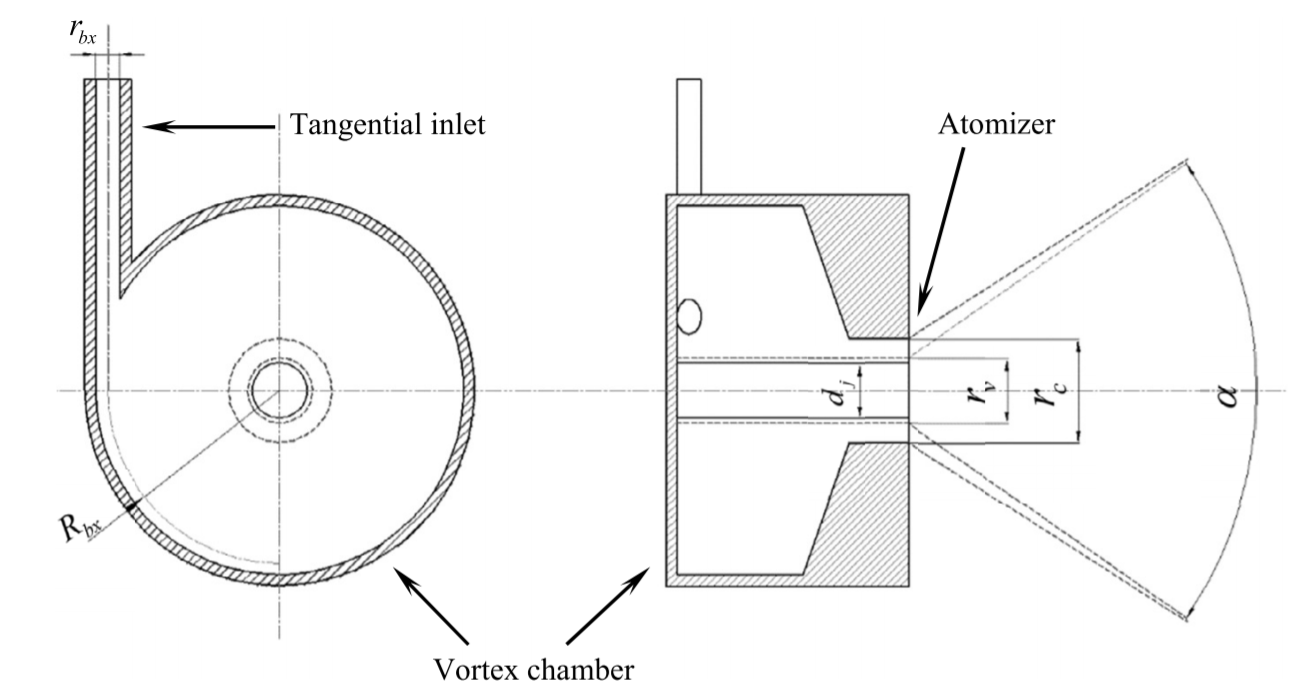
\includegraphics[width=\linewidth]{swirl}
    \caption{Cross section of a swirl injector}
\end{figure}

The schematic before shows how a swirl injector works. We see that there is only few parameters to take  into account to design this kind of injector. 


\section{Feeding system}
After having designed most of our propulsion system. We need to carefully link them by designing our feeding system. The biggest challenge is to create a system that will both fit in our spacecraft and deliver the right amount of propellant from the tanks to the engine through our different, required other subsystems.\\

The general pressure loss in a system is given by :

$$
\Delta P = K\frac \rho 2 w^2
$$

With $K$ depending on the type of change in system geometry as follow : 
\begin{figure}[H]
	\centering
	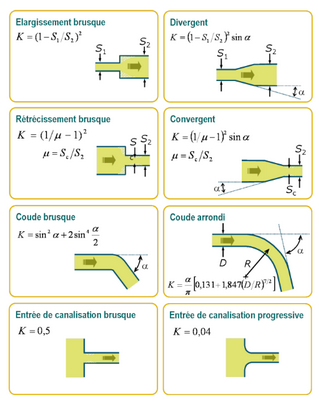
\includegraphics[height=12cm]{pertecharge}
	\caption{$K$ values for geometry changes}
\end{figure}
In our case, we will use the progressive line entering loss $K = 0.04$ and the bends $ K(\alpha) = \sin^2(\alpha) + 2\sin^4\bigg(\frac\alpha 2\bigg)$. Another $K$ will also be used for the entrance of the injector, which will be specified later on.\\

For manufacturing costs and simplicity purposes, we choose to only use $45^\circ$ bends which will result in $K_{bends}=0.5429$.\\

With that and the length measurements in mind, we designed the following feeding system layout for which we will then calculate the pressure variations along it :
\begin{figure}[H]
	\centering
	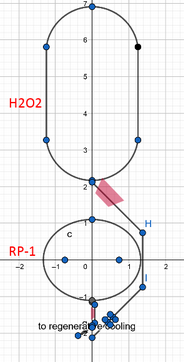
\includegraphics[height=10cm]{feeding}
	\caption{Feeding system layout (To scale)}
\end{figure}
\begin{figure}[H]
	\centering
	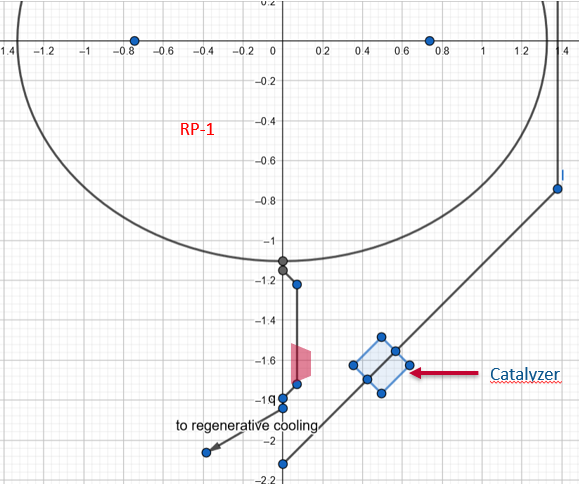
\includegraphics[height=8cm]{feedingzoom}
	\caption{Feeding system layout - Zoomed (To scale)}
\end{figure}
\subsection{Line diameters}
In order to choose our line diameters, we can first use our volume flow and then get the line area from it and then at the end, the line diameter.\\
\underline{Fuel} 
\begin{align}
\dot{V_f}&= \frac{\dot{m_f}}{\rho_f} = 0.0015298m^3/s\\
A_{line_f} &= \frac{\dot V_f}{w_f}=5.21\times 10^{-5} mm^2\\
d_{line_f} &= 2\sqrt{\frac{A_{line_f}}{\pi}} = 8.1447mm
\end{align}
As we are trying to insure a high injection velocity and to insure a certain margin in pressure and velocity, we will choose a line diameter of $7$ mm for the fuel feeding system.
\underline{Oxidizer}
\begin{align}
\dot{V_o}&= \frac{\dot{m_o}}{\rho_o} = 0.006042m^3/s\\
A_{line_o} &= \frac{\dot V_o}{w_o}=0.000275 mm^2\\
d_{line_o} &= 2\sqrt{\frac{A_{line_o}}{\pi}} = 18mm
\end{align}
In this case, we will choose a line diameter of $15$ mm for the oxidizer.

\subsection{Fuel feeding system}
The following items in our fuel feeding system will cause pressure drops :
\begin{itemize}
	\item Tank exit : $K=0.04$
	\item 4 $\times$ $45^\circ$ bends : $K = 0.5429$ for each
	\item Straight line losses : $\Delta P = \frac \rho 2 w^2 f \frac{L}{D}$
	\item Friction coefficient : $f = 0.02$
	\item Regenerative cooling : $\Delta P = 0.25$ bar
	\item Fuel injection : $\Delta P = 9.3843$ bars
\end{itemize}

With our current layout, we have $5$ straight lines which will cause pressure losses on the fuel side. Three of them are before the turbopump which is placed at the end of the third straight section, right before the third bend. We consider a velocity of $8$ m/s before the turbopumps and of $v_{inj}=29.363$ m/s after. The line loss for each section is given by : 
$$
\Delta P = \frac {810} 2 w^2 \times 0.02 \times \frac{L_{section}}{0.007}
$$
\begin{enumerate}
	\item First section ($L_{section}=0.05m$) : $\Delta P = 0.037029$ bar
	\item Second section ($L_{section}=0.1m$) : $\Delta P = 0.074057$ bar
	\item Third section ($L_{section}=0.5m$) : $\Delta P = 0.37029$ bar
	\item Fourth section ($L_{section}=0.1m$) : $\Delta P = 0.997699$ bar
	\item Fifth section ($L_{section}=0.05m$) : $\Delta P = 0.49884$ bar
\end{enumerate}
There are also two different values for the bend losses depending on the position of the bend (before or after the turbopump), we have $2$ of each :
\begin{itemize}
	\item $\Delta P_{before} = 0.14072 $ bar
	\item $\Delta P_{after} = 1.8957$ bar
\end{itemize}
The tank exit loss is :
$$
\Delta P_{exit} = K_{exit} \times \frac{\rho_F}2 \times 8 ^ 2 = 0.010368\text{ bar}
$$
\subsection{Oxidizer feeding system}
The following items in our oxidizer feeding system will cause pressure drops :
\begin{itemize}
	\item Tank exit : $K=0.04$
	\item 4 $\times$ $45^\circ$ bends : $K = 0.5429$ for each
	\item Straight line losses : $\Delta P = \frac \rho 2 w^2 f \frac{L}{D}$
	\item Friction coefficient : $f = 0.02$
	\item Catalyzer : $\Delta P = $ bars
	\item Oxidizer injection : $\Delta P = 4.9599$ bars
\end{itemize}

On this part of the feeding system, we also have $5$ sections and $4$ bends of $45^\circ$ each. We also consider a velocity of $8$ m/s before the turbopump and $21.971$ m/s after. However, due to the larger distances (due to our tank layout), the turbopump's position in the feeding system is different and is now positioned after the first bend, right at the beginning of the second straight line. This results in $3$ bends being at high velocity and $1$ at relatively slower velocity.\\

Here, each straight line loss section is given by : 
$$
\Delta P = \frac {1450} 2 w^2 \times 0.02 \times \frac{L_{section}}{0.015}
$$
With : 

\begin{enumerate}
	\item First section ($L_{section}=0.05m$) : $\Delta P = 0.030933$ bar
	\item Second section ($L_{section}=1.95m$) : $\Delta P = 9.0992$ bars
	\item Third section ($L_{section}=1.4836m$) : $\Delta P = 6.9228$ bars
	\item Fourth section ($L_{section}=1.15m$) : $\Delta P = 5.3662$ bars
	\item Fifth section ($L_{section}=0.6m$) : $\Delta P = 2.7997$ bars
\end{enumerate}

For the bends, we have :

\begin{itemize}
	\item $\Delta P_{before} = 0.2519 $ bar ($1$ of them)
	\item $\Delta P_{after} = 1.0614$ bar ($3$ of them)
\end{itemize}

The tank exit loss is :
$$
\Delta P_{exit} = K_{exit} \times \frac{\rho_o}2 \times 8 ^ 2 = 0.01856\text{ bar}
$$
\section{Turbo pumps}
As most of our subsystems have a defined pressure drop due to their specific design, we have made the choice to use this feeding system design with all losses included to then design our turbopumps to have a pressure rise in accordance with our pressure requirements. We chose to go with electrically driven turbo pumps as we have a good amount of electrical power since we use fuel cells in our spacecraft.\\

Our respective turbopump required created pressures are : 
\begin{itemize}
	\item Fuel side : $\Delta P_{T_f} = P_{Chamber} + \Delta P_{feeding_f} + \Delta P_{inj_f} + \Delta P_{Regenerative\ cooling} - P_{Tank_f}$
	\item Oxidizer side : 	$\Delta P_{T_o} = P_{Chamber} + \Delta P_{feeding_o} + \Delta P_{inj_o} + \Delta P_{Catalyzer} - P_{Tank_o}$
\end{itemize}
Thus,
\begin{align}
\Delta P_{T_f} &= 54.395\ \text{bars}\\
\Delta P_{T_o} &= 102.28\ \text{bars}
\end{align}
Considering an efficiency of $0.9\times 0.75$, with $0.9$ for the electrical part and $0.75$ for the mechanical part, we get the following powers :
\begin{align}
	Power_{fuelpump} &=\dot{m_f}\frac{P_{T_f}}{\rho_F \eta} = 13\ 461\ W\\
	Power_{Oxpump} &= \dot{m_o}\frac{P_{T_o}}{\rho_o \eta} = 96\ 030\ W
\end{align}
Considering a maximum continuous burn time of $900$ seconds, we get the following energy with a 40\% margin as we are still unsure about the performance of such turbopump :\\
\begin{equation}
	E_{kWh} = \frac{(Power_{fuelpump} + Power_{Oxpump})\times 900}{3.6\times 10^6} = 38.322\ kWh
\end{equation}

We also know the following vapor pressures :
\begin{itemize}
	\item $H_2O_2$ : $666.612$ Pa at $30^\circ$ C
	\item $RP-1$ : $700$ Pa between $20^\circ$C and $25^\circ$ C
\end{itemize}
With the information we have, we can calculate the pump head rise and the NPSH.
\begin{align}
	H_{p_{Fuel}} &= \frac{\Delta p_{p_{Fuel}}}{g_0 \rho_{Fuel}} = 747.474\ m\\
	H_{p_{Ox}} &= \frac{\Delta p_{p_{Ox}}}{g_0 \rho_{Ox}} = 754.192\ m\\
	NPSH_{Fuel} &= \frac{p_{i_{Fuel}} - p_{v_{Fuel}}}{g_0 \rho_{Fuel}} = 6.569\ m\\
	NPSH_{Ox} &= \frac{p_{i_{Ox}} - p_{v_{Ox}}}{g_0 \rho_{Ox}} = 7.0465\ m
\end{align}
We can then get the number of stages :
\begin{equation}
	n= 1 +floor(\frac{\Delta p_p}{\Delta p_{ps}})
\end{equation}
Thus, using $\Delta p_{ps} = 47\times 10^6\ Pa$,
\begin{align}
	n_{Fuel} &= 126\ 373
	n_{Ox} &= 228\ 256
\end{align}
We can also get the rotation speeds :
\begin{align}
	N_{Fuel} &= 1.636\ rad/s = 15.623\ RPM\\
	N_{Ox} &= 0.532\ rad/s = 5.079\ RPM
\end{align}
Then
\begin{align}
	u_{t_{Fuel}} &= \sqrt{\frac{gH_{p_{Fuel}}}{n\psi}}=0.325\ m/s\\
	u_{t_{Ox}} &= \sqrt{\frac{gH_{p_{Ox}}}{n\psi}} =0.243\ m/s\\
	D_{2t_{Fuel}} &=\frac{u_{t_{Fuel}}}{N_{r_{Fuel}}}= 0.199\ m\\
	D_{2t_{Ox}} &= \frac{u_{t_{Ox}}}{N_{r_{Ox}}} 0.457\ m\\
	D_{1t_{Fuel}} &= \sqrt[3]{\frac{\frac{4}{\pi}Q_{Fuel}}{\phi N_{r_{Fuel}}(1-L^2)}} = 2.197\ m\\
	D_{1t_{Fuel}} &=\sqrt[3]{\frac{\frac{4}{\pi}Q_{Ox}}{\phi N_{r_{Ox}}(1-L^2)}} = 6.131\ m
\end{align}
\section{Pressure evolution summary}
\subsection{Fuel side}
\begin{table}[H]
	\centering
\begin{tabular}[H]{|c|c|c|}
	\hline
	\cellcolor{gray!50}Contributor& \cellcolor{gray!50}Pressure Drop (bars) & \cellcolor{gray!50}Pressure at the end of this part (bars)\\
	\hline
	Tank & NA & $1.3$ \\
	\hline
	Tank exit & $0.010368$ & $1.29$\\
	\hline
	First section & $0.037$ &$1.253$\\
	\hline
	First bend &$0.14$ &$1.113$\\
	\hline
	Second section &$0.074$ &$1.039$\\
	\hline
	Second bend &$0.14$ &$0.899$\\
	\hline
	Third section &$0.37$ &$0.529$\\
	\hline
	Turbo pump & $54.395 $ (Rise) &$59.924$\\
	\hline
	Valve & $5$ &$54.924$\\
	\hline
	Third bend &$1.8957$ &$53.0283$\\
	\hline
	Fourth section &$0.997$ &$52.0313$\\
	\hline
	Fourth bend &$1.8957$ &$50.1356$\\
	\hline
	Fifth section &$0.499$ &$49.6366$\\
	\hline
	Cooling &$0.25$ &$49.3866$\\
	\hline
	Injection &$9.38$ &$40.0066$\\
	\hline
	Combustion chamber & NA &$40.0066$\\
	\hline
\end{tabular}
\caption{Pressure evolution on fuel side}
\end{table}
\begin{figure}[H]
	\centering
	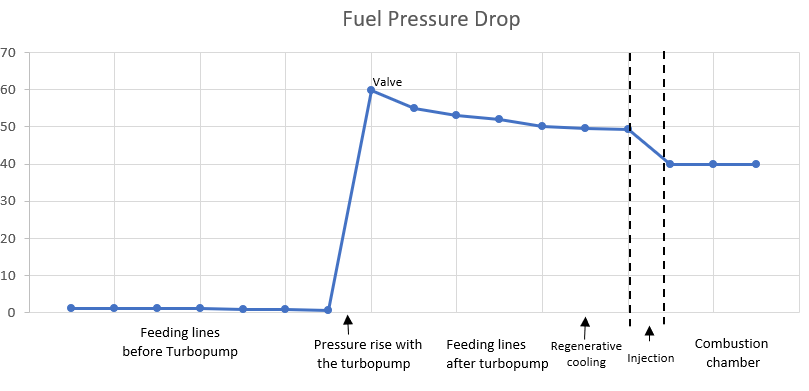
\includegraphics[width=\linewidth]{fuelchart}
	\caption{Pressure evolution on fuel side (bars)}
\end{figure}
\subsection{Oxidizer side}
\begin{table}[H]
	\centering
\begin{tabular}[H]{|c|c|c|}
	\hline
	\cellcolor{gray!50}Contributor& \cellcolor{gray!50}Pressure Drop (bars) & \cellcolor{gray!50}Pressure at the end of this part (bars)\\
	\hline
	Tank & NA & $1.3$ \\
	\hline
	Tank exit & $0.010368$ & $1.29$\\
	\hline
	First section & $0.031$ &$1.259$\\
	\hline
	First bend &$0.25$ &$1.009$\\
	\hline
	Turbo pump & $102.28 $ (Rise) &$108.289$\\
	\hline
	Turbo pump & $5$ &$103.289$\\
	\hline
	Second section &$9.09$ &$94.199$\\
	\hline
	Second bend &$1.06$ &$93.139$\\
	\hline
	Third section &$6.9228$ &$86.2162$\\
	\hline
	Third bend &$1.06$ &$85.1562$\\
	\hline
	Fourth section &$5.366$ &$79.7902$\\
	\hline
	Fourth bend &$1.06$ &$78.7302$\\
	\hline
	Fifth section &$2.7997$ &$75.9305$\\
	\hline
	Catalyzer &$30.95$ &$44.9805$\\
	\hline
	Injection &$4.96$ &$40.0205$\\
	\hline
	Combustion chamber & NA &$40.0205$\\
	\hline
\end{tabular}
\caption{Pressure evolution on fuel side}
\end{table}
\begin{figure}[H]
	\centering
	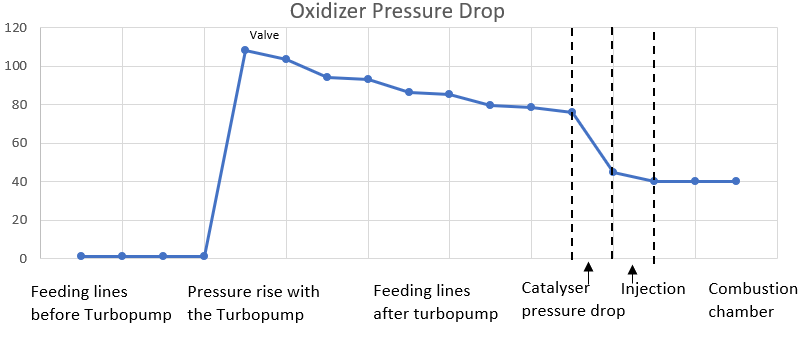
\includegraphics[width=\linewidth]{oxchart}
	\caption{Pressure evolution on oxidizer side (bars)}
\end{figure}
\section{Engine}
\section{Nozzle}

\chapter{Simulations}
\qquad \underline{By} : Lukas
\label{chap:sim}
\section{Engine performance simulation}
\qquad In order to simulate the engine performance, the largest single burn was simulated. As the initial burn for entering a Geostationary Transfer Orbit would require more than $900$ s of engine burn time due to the large starting mass of the spacecraft, roughly half of this initial burn was simulated. An immediate result of the requirement to limit engine burn time to $900$ s is therefore, that the first burn needs to be split into two burns. The engine simulation aims to determine thrust, acceleration, $\Delta v$ and propellant masses over time. A combined MATLAB$^{\mbox{\scriptsize{\textregistered}}}$  / Simulink$^{\mbox{\scriptsize{\textregistered}}}$  was used, calculating thrust based on following equation:
\begin{equation}
	F = \dot m \times C_F \times C^*\\
\end{equation}

with : 
$$
C^* = \frac{p_c\times A_t}{\dot{m}}
$$

and

$$
C_F = \sqrt{\frac{2\times \kappa^2}{\kappa - 1}\times \bigg(\frac{2}{\kappa + 1}\bigg)\times\bigg[1 - \bigg(\frac{p_e}{p_c}\bigg)^{\frac{\kappa - 1}{\kappa}}\bigg]} + \varepsilon\bigg(\frac{p_e-p_a}{p_c}\bigg)
$$

assuming a constant mass flow rate of $\dot{m} = 10$ kg/s. Considering a constant chamber pressure after initial start-up of $40$ bars and an exit pressure of $3900$ Pa, which was determined using RPA, a steady-state thrust of $33.6$kN was observed, as can be seen in \autoref{fig1}. $\kappa$ was determined using RPA as well and, while varying slightly throughout the engine, assumed as constant to facilitate the simulation.

\begin{figure}[H]
	\centering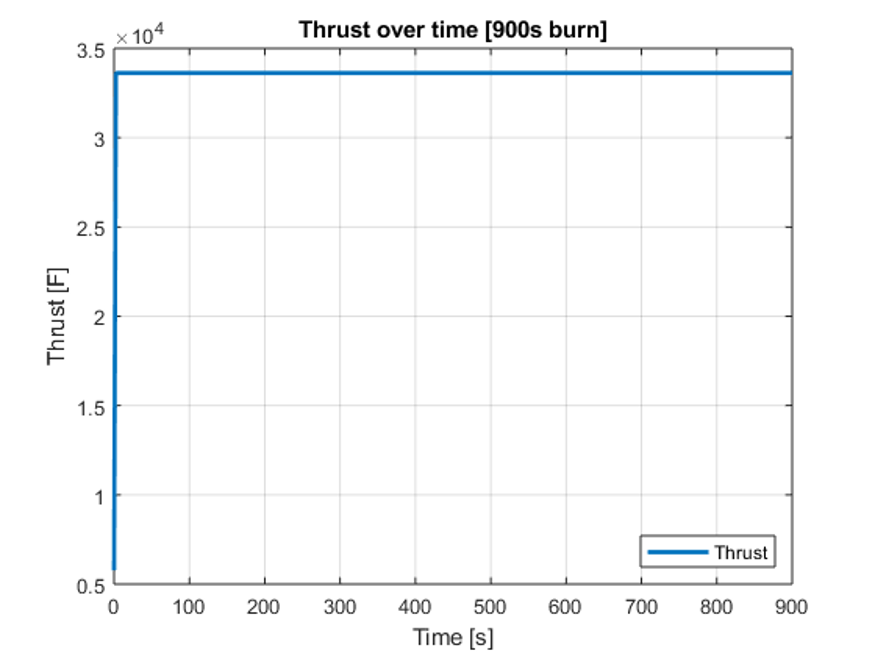
\includegraphics[width=0.9\linewidth]{thrusttime}
	\caption{Engine simulation - Thrust over time}\label{fig1}
\end{figure}

The resulting acceleration and $\Delta v$ over time are shown in \autoref{fig2}.
\begin{figure}[H]
	\centering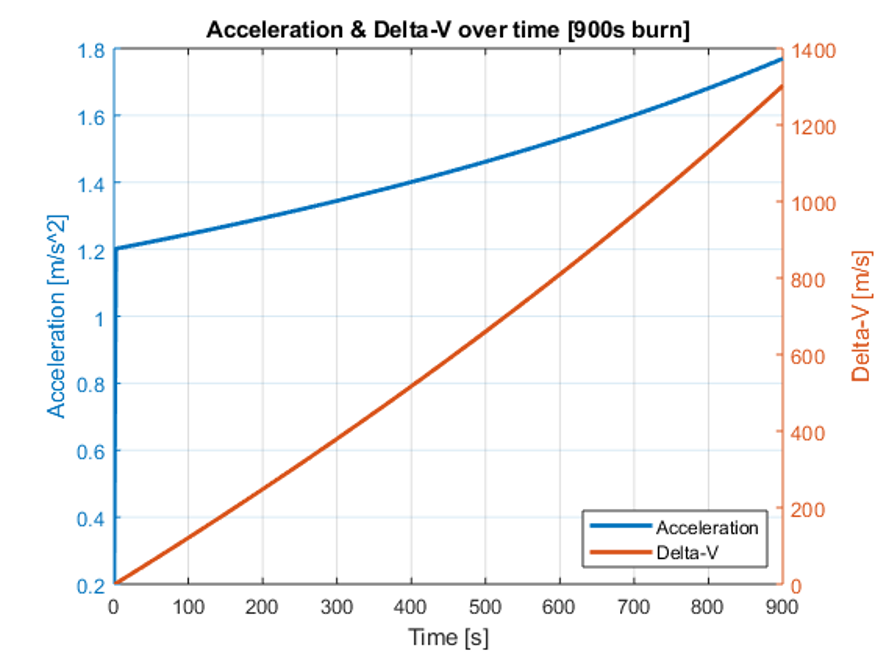
\includegraphics[width=0.9\linewidth]{accdeltav}
	\caption{Engine simulation - Acceleration and $\Delta v$ over time}\label{fig2}
\end{figure}

The acceleration, shown in blue, starts off at around $1.2$ m/s$^2$, which is a value in the range of our expectations. After $900$ seconds, the mass loss leads to a final acceleration of slightly below $1.8$ m/s$^2$, when a $\Delta v$ of ca. $1\ 300$ m/s is reached. At the point of discovery of the insufficiency of $900$ s, the decision to divide the first burn into two was taken. 
Lastly, the behavior of the propellant masses is portrayed in \autoref{fig3}. 

\begin{figure}[H]
	\centering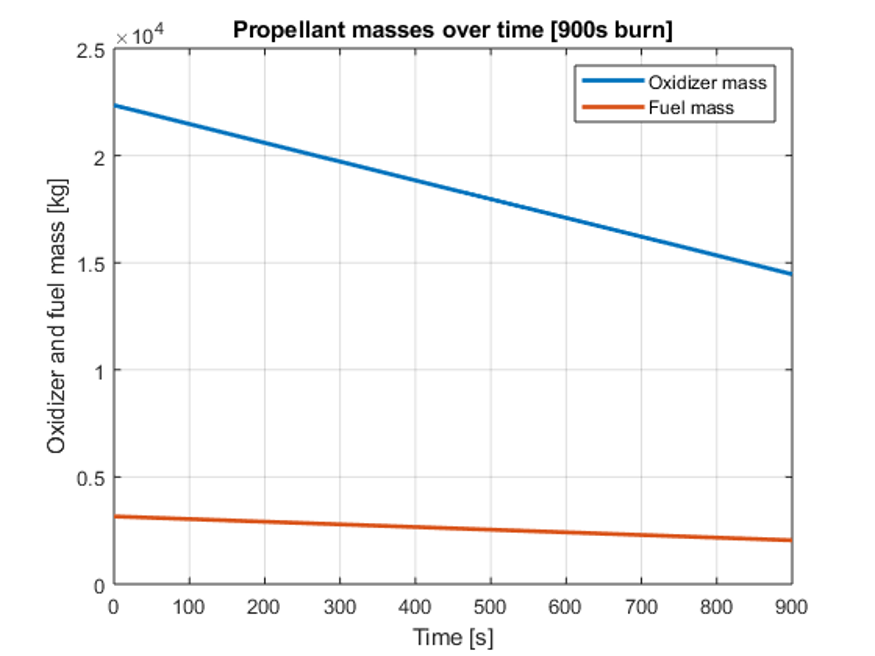
\includegraphics[width=0.9\linewidth]{propmasstime}
	\caption{Engine simulation - Propellant masses over time}\label{fig3}
\end{figure}

With roughly one third of the total usable propellant having been burnt throughout 900 seconds of burn time, these results are also according to expectations. The simulation of the maximum burn time is representative of the entirety of burns throughout the mission, therefore it validates the viability of the engine design for the fulfillment of mission requirements. The complete simulation script and model can be found in the annex. \pagebreak 
\section{Regenerative cooling simulation}

\qquad The thermal loads of the engine combustion are managed by regenerative cooling of the engine, with the cooling channels running along axial lines throughout the entire length of the engine. The cooling liquid is the engine fuel (RP-1), being fed into the combustion chamber wall and running along cooling channels with varying cross-section area before exiting at the end of the nozzle. The cooling channel design was determined by simulation of the relevant wall temperatures in steady-state operation, where a temperature at a given location does not change over time, with heat flux in and out being equal. Following assumptions and design choices were made before and during the preliminary calculations:
\begin{itemize}
	\itemsep0em 
	\item	The inner engine wall is made of copper throughout the entire engine
	\item	The outer wall is made of steel
	\item	A defined number of symmetrical rectangle-shaped cooling channels run through the engine wall, with varying cross-section to allow for higher and lower thermal flux at different sections
	\item	The cooling channels are symmetrical w.r.t. to the engine propellant flow axis
	\item	Injection into the cooling channels takes place at the combustion chamber end of the engine, in order to create larger heat transfer at more thermally stressed areas due to lower coolant temperature
	\item	\textbf{The RP-1 is assumed to not change phase during the regenerative cooling} (While this decreases simulation accuracy, too little data on high-pressure RP-1 phase change behaviour was available. The temperature does however affect the liquid’s heat capacity within the simulation)
\end{itemize}

In order to simulate the steady-state thermal behaviour of the engine along its length, some simplifications needed to be conducted. All coefficients (e.g. ratio of specific heat capacities) are assumed to be constant throughout each section, with three different values for the combustion chamber, throat area and nozzle respectively. In addition, all time-related values were transformed into distance-based values, so that the simulation time is actually millimetres, instead of seconds. This was achieved by limiting the simulation time to the engine length in millimetres and using switches to change constants based on what section the propellant is in at any given millimetre value, while using the flow velocity as the key parameter to transform into metres. The simulation script, model and complete results can be found in the annex. At this point, only some key conclusions will be presented and discussed.\\

The central aim of the iterative calculation was to determine a combination of material, wall thickness and cooling channel geometry which allows the inner wall temperature to remain below its maximum operating temperature. All other temperatures, like the coolant and outer wall temperatures, were of secondary importance. Due to its high thermal conductivity, copper was chosen as the inner wall material.

 The cooling channel cross-section was defined to always be equally sized relative to the local engine diameter, with the ratio being a function of the local engine wall cross-section area and a factor, which represents the filling grade. \autoref{fig4} shows the cross-section change over the engine length. The rectangular geometry is defined by a ratio of width to height of $5$.

\begin{figure}[H]
	\centering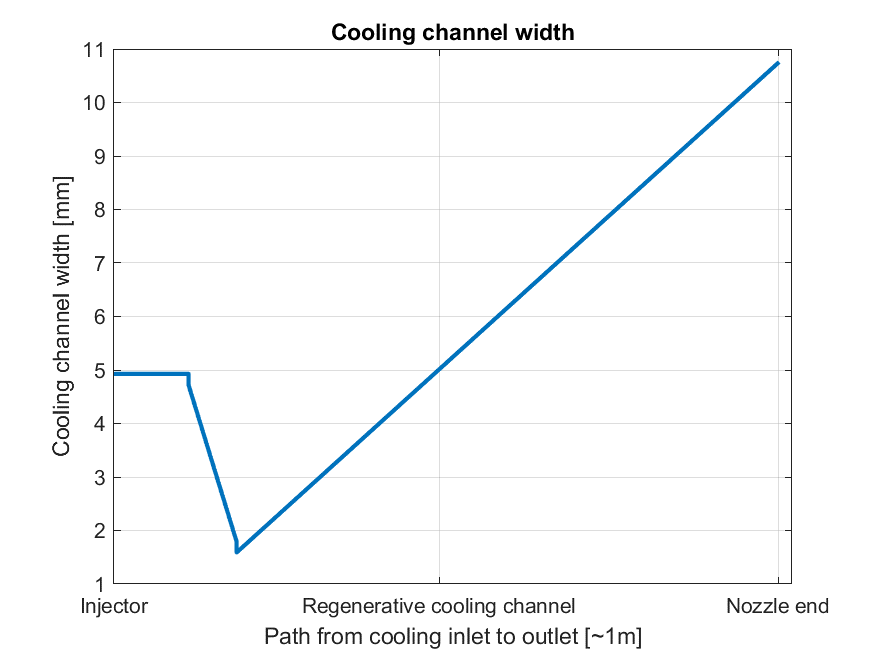
\includegraphics[width=0.9\linewidth]{coolingchannelwidth}
	\caption{Regenerative cooling simulation - Cooling channel width over engine length}\label{fig4}
\end{figure}

The final cooling channel system is a compromise between the copper wall temperature and minimum necessary material for weight savings. Therefore, the copper wall has a thickness of $6$ mm in the combustion chamber, $7$ mm in the throat area and $5$ mm in the nozzle section. The resulting relevant temperatures can be seen in \autoref{fig5}.

\begin{figure}[H]
	\centering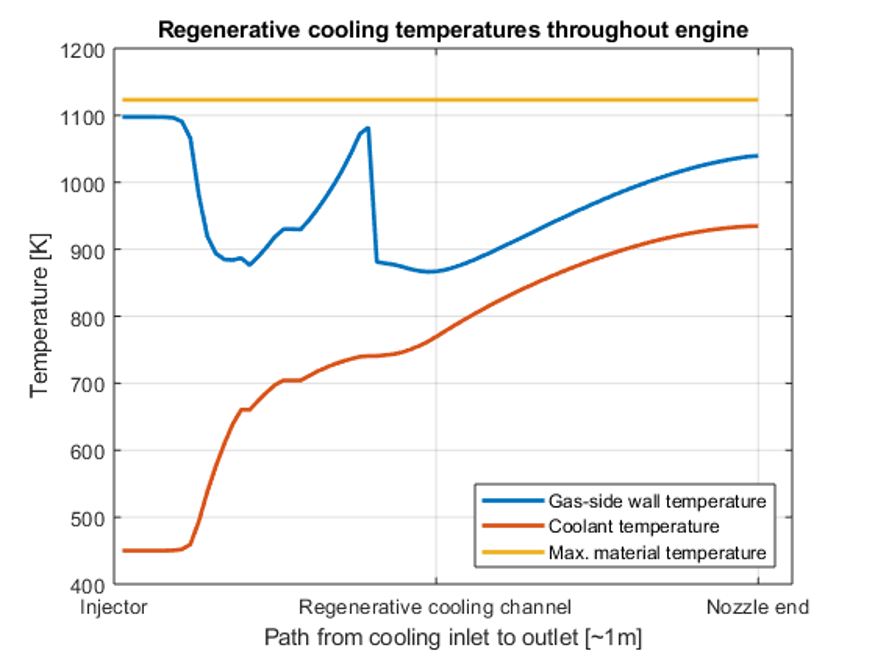
\includegraphics[width=0.9\linewidth]{relevanttemps}
	\caption{Regenerative cooling simulation - Relevant temperatures}\label{fig5}
\end{figure}

The highest temperatures can be observed in the combustion chamber section, as low flow speeds cause less convective heat transfer to take place, reducing the overall heat flux. The gas-side wall temperature then drops in the beginning of the throat area, before rising again towards the throat. After passing the throat, the gas-side wall temperature drops sharply and then rises again towards the nozzle exit.
\section{Hydrogen peroxide decomposition simulation}
\label{sec:11-3}
\qquad As mentioned in \autoref{sec:10-3}, the decomposition of hydrogen peroxide is used for self-pressurization of the oxidizer tank as well as power generation in a fuel cell in combination with hydrogen. As hydrogen peroxide is not only decomposing, but the decomposition is also an exothermal process, the thermal control system needs to be well under control in order to avoid critical behavior of the hydrogen peroxide if $150^\circ$ C are exceeded. Therefore, a detailed simulation has been performed, taking wall thicknesses, materials, radiative and absorbing coefficients as input parameters. The simulation is structured like a control system, calculating the temperature of the hydrogen peroxide inside the tank, the cold and hot wall temperatures. Upon reaching the specified target temperature, the control loop rotates the spacecraft to a neutral degree for constant hydrogen peroxide temperature. Before discussing the results, an overview of the simplifications taken for facilitation of the simulation follows:
\begin{itemize}
	\itemsep0em 
	\item	Inside the tank, only vaporization takes place, no condensation
	\item	The space craft can rotate to any angle instantaneously and there is no modelling of the necessary thruster activation
	\item	The cold and hot walls are always at a homogenous temperature, only depending on heat flux between hydrogen peroxide, the walls, the sun and dark space
	\item	As the structural calculations needed to be complete before the simulation was able to prove the technical feasibility of the decomposition regulation, \textbf{the hydrogen peroxide tank is assumed to be made of only one material throughout the rest of the documentation, while the simulation allows for two different materials}, as different heat flux coefficients are advantageous. Therefore, the results of this simulation are not exactly compatible with the final space craft design and more of a proof of concept, to be reunited with the structural design as a next step.
\end{itemize}

The simulation showed that, with the simplifications taken, a control system maintaining the hydrogen peroxide pressure at an acceptable level is technically feasible. A control reaction to raising the temperature from $310$ K to $350$ K has been chosen as the case for technical feasibility demonstration. As explained in \autoref{sec:10-3}, the rotational angle of the space craft is the dictating parameter for heat input and output. \autoref{fig6} shows the rotational angle, resulting H2O2 pressure, the relevant temperatures and the generated energy considering consumption of all generated oxygen in the fuel cell. The four graphs are outputs of the same simulation, the complete script and model for which can be found in the annex. The initial values for the integration blocks, which output temperatures, are all assumed.

\begin{figure}[H]
	\centering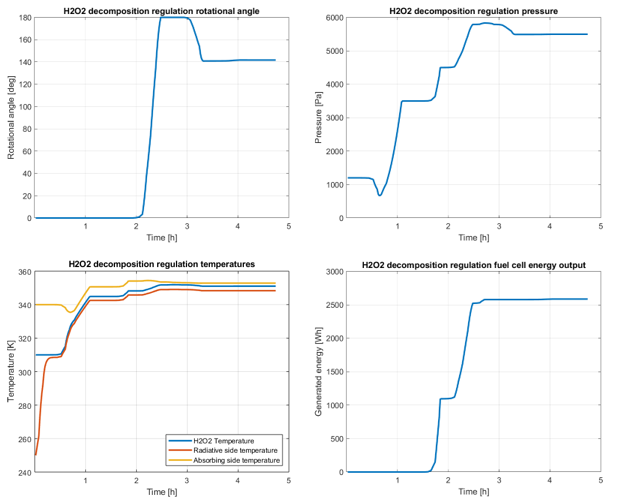
\includegraphics[width=\linewidth]{feasibility}
	\caption{Demonstration case for technical feasibility of $H_2O_2$ decomposition regulation}\label{fig6}
\end{figure}
As the simulation results show, the rotational angle is initially maintained at $0^\circ$, meaning full exposure of the more absorbing side towards the sun, with the less radiative side facing dark space. After $2$ hours, the space craft turns towards the other side, decreasing the heat flux gradually while approaching the target temperature. In the end, a constant neutral rotational angle of $140^\circ$ is maintained, with a final control error of around $1-2$ K. After this process, $2,5$ kWh of energy were generated, while the pressure inside the tank has risen from around $1000$ Pa to $5500$ Pa. The tank pressure is determined via interpolation of temperature-dependent vaporization pressures to gain a function of pressure with respect to temperature.
\chapter{Evaluation}
\section{Requirement verification}
\section{Lessons learnt}
%\chapter*{Conclusion}



%\begin{acronym}[EHPAD] % Give the longest acronym here

%\end{acronym}

\listoffigures

\listoftables
\nopagebreak
\chapter*{Annexes}
\section*{Annex I - Gantt Diagramm}
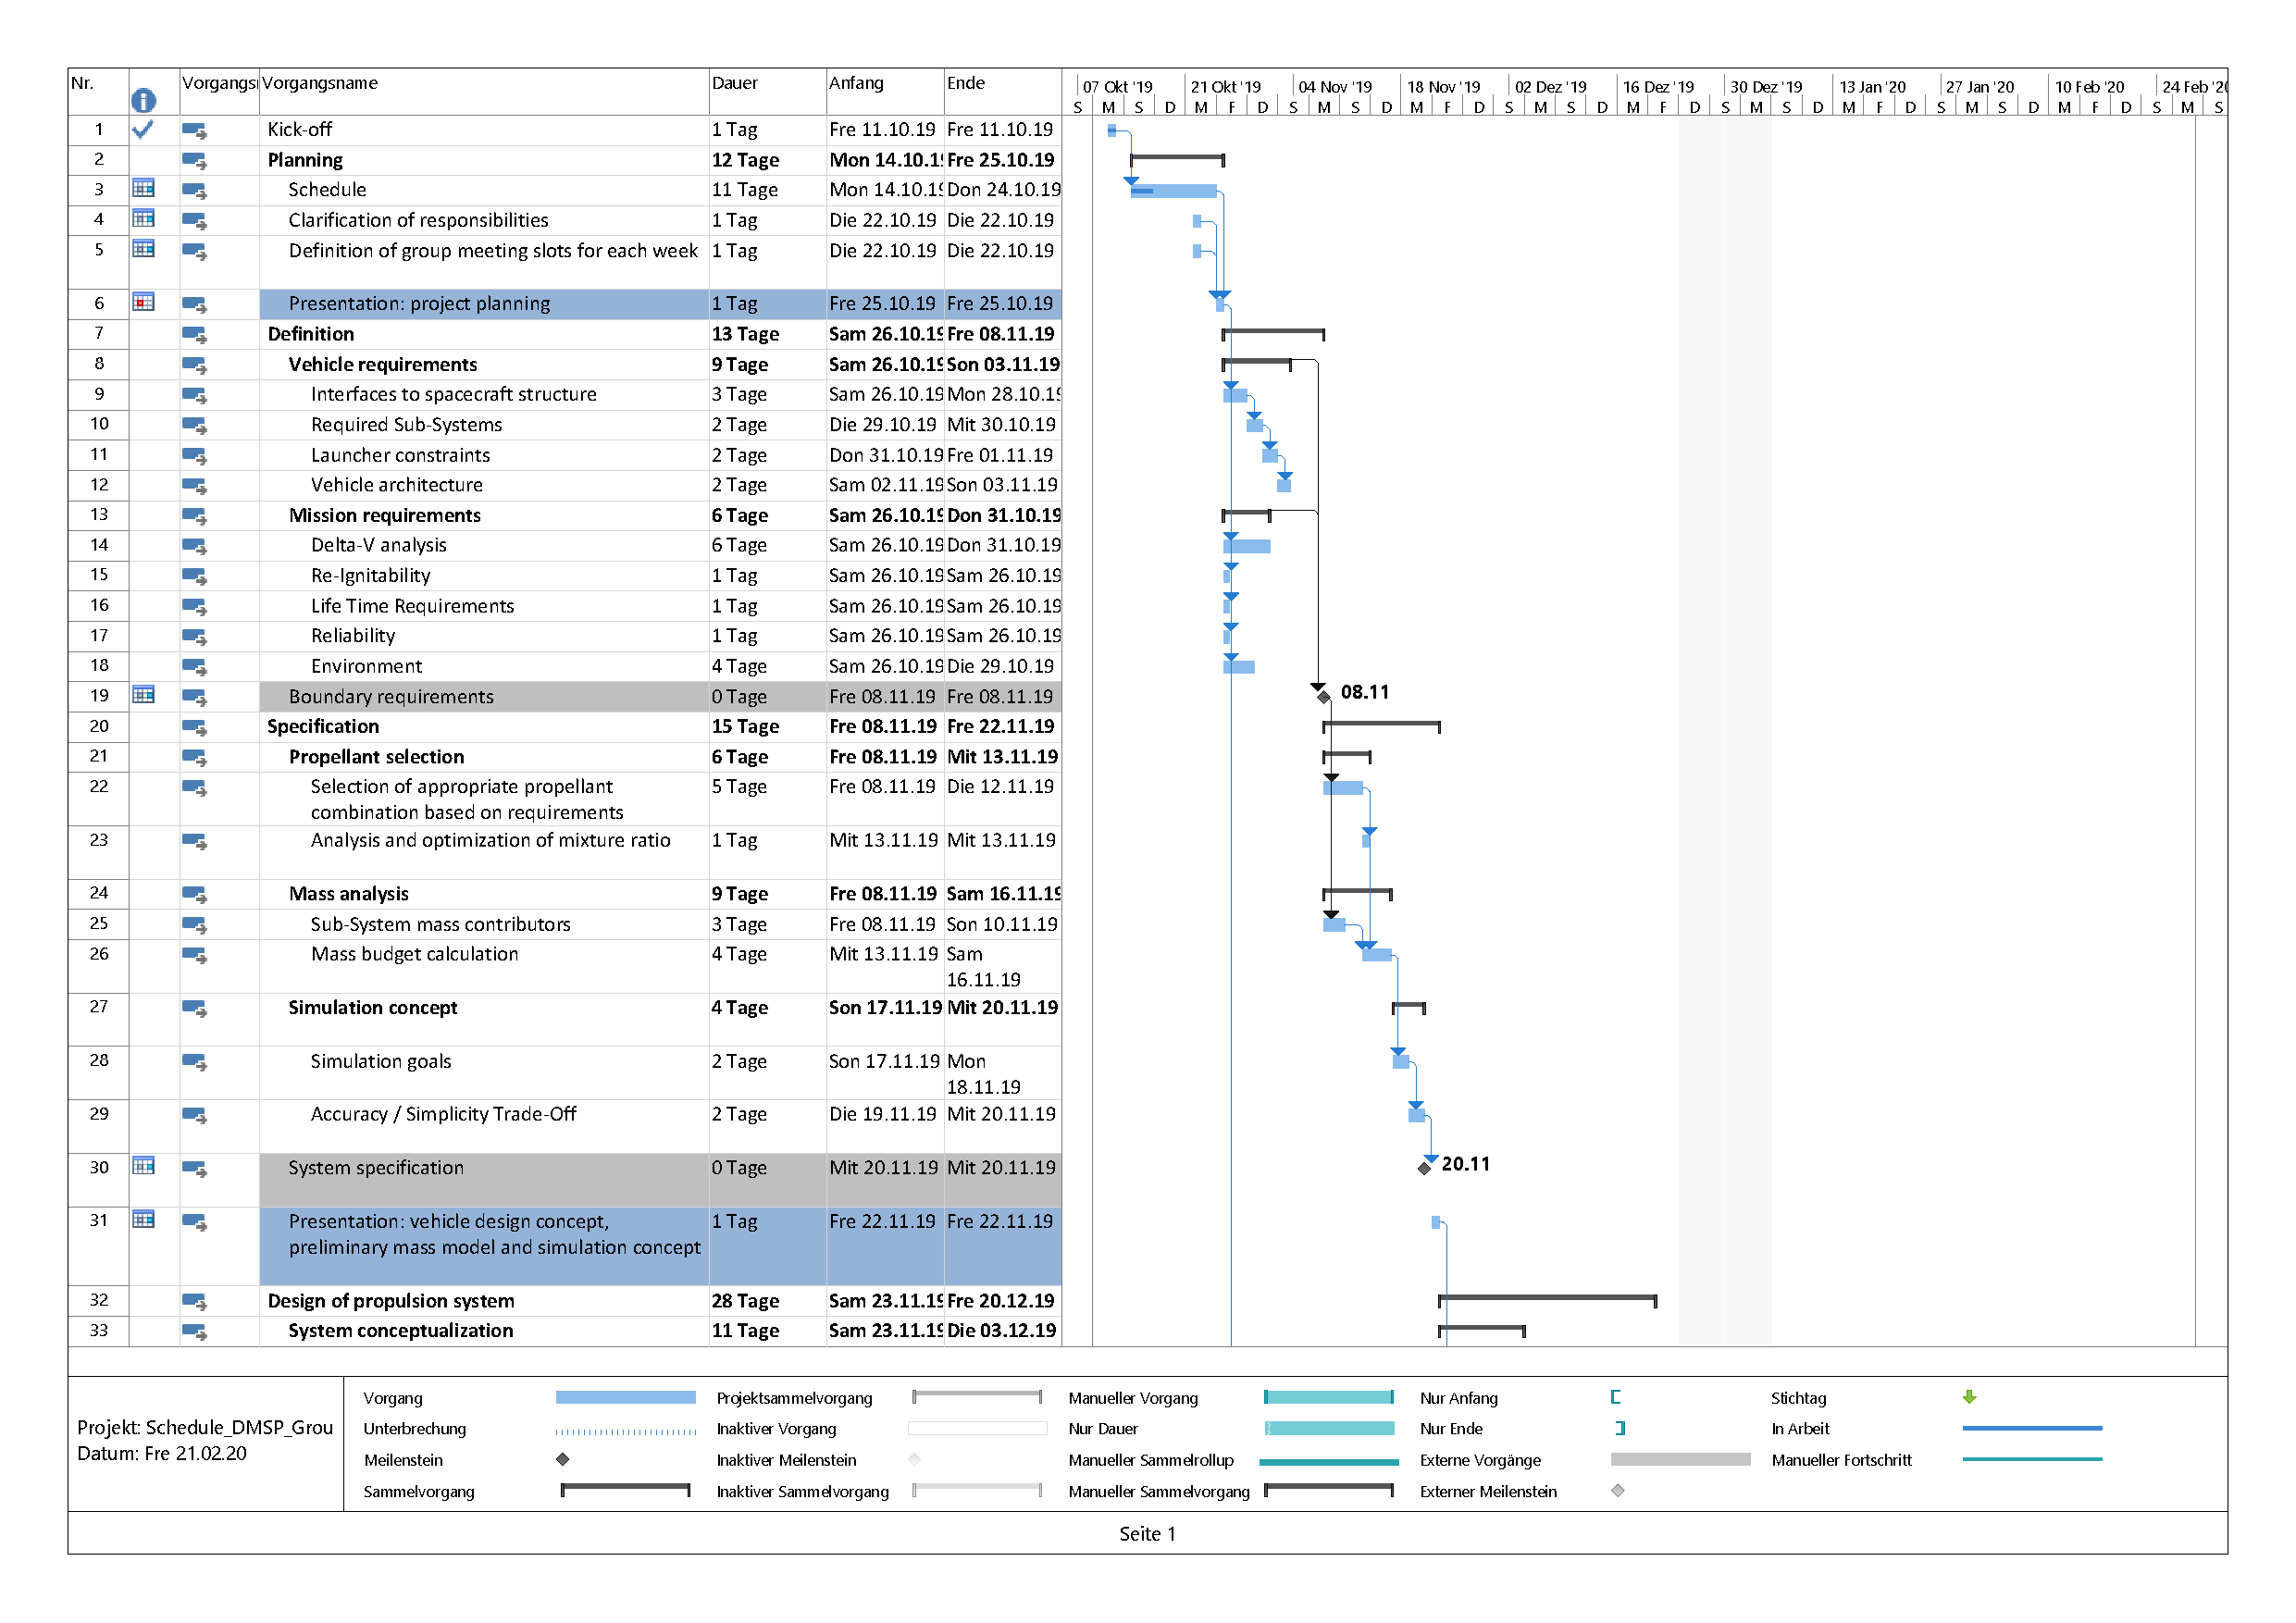
\includepdf[pages=-]{Gantt}\label{Gantt}


\chapter*{Sources}

\begin{enumerate}
	\itemsep0em 
	\footnotesize{
	\item http://braeunig.us/space/propel.htm
	\item http://astronautix.com/l/loxkerosene.html
	\item https://en.wikipedia.org/wiki/Liquid\_rocket\_propellant\#Bipropellants
	\item http://www.astronautix.com/h/h2o2kerosene.html
	\item Hydrogen Peroxide / Kerosene, Liquid-Oxygen / Kerosene, and Liquid-Oxygen / Liquid
	Methane for Upper Stage Propulsion, Paper, S. Krishnan* Universiti Teknologi Malaysia
	\item https://ntrs.nasa.gov/archive/nasa/casi.ntrs.nasa.gov/19720019028.pdf
	\item https://www.nasa.gov/centers/glenn/technology/fuel\_cells.html
	\item https://www.ginerinc.com/regenerative-fuel-cell-systems
	\item https://ntrs.nasa.gov/archive/nasa/casi.ntrs.nasa.gov/19990063763.pdf
	\item http://www.esa.int/esapub/bulletin/bullet90/b90dudle.htm
	\item https://www.sciencedirect.com/science/article/abs/pii/S0360319904003106
	\item http://citeseerx.ist.psu.edu/viewdoc/download?doi=10.1.1.526.3797\&rep=rep1\&type=pdf
	\item http://juser.fz-juelich.de/record/135459/files/HP3d\_3\_Ranjbari.pdf
	\item https://www.sciencedirect.com/topics/chemistry/proton-exchange-membrane-fuel-cells
	\item http://www.dartmouth.edu/~cushman/courses/engs37/FuelCells.pdf
	\item https://ocw.mit.edu/courses/aeronautics-and-astronautics/16-851-satellite-engineering-fall-2003/le
	cture-notes/l3\_scpowersys\_dm\_done2.pdf
	\item Article : The design and main performance of a hydrogen peroxide/kerosene coaxial-swirl injector in a lab-scale rocket engine
	\item Article : Design and Analysis of a Fuel Injector of a Liquid
	Rocket Engine
	\item Article : The spray characteristic of gas-liquid coaxial swirl injector by experiment
	\item https://www.grc.nasa.gov/www/k-12/airplane/shaped.html
	\item TPSX NASA Material Properties Database : https://tpsx.arc.nasa.gov/ 
	\item Columbia accident report : https://www.nasa.gov/columbia/home/CAIB\_Vol1.html
	\item  An Internet Book on Fluid Dynamics - The Flat Plate Airfoil :\\http://brennen.caltech.edu/fluidbook/externalflows/lift/flatplateairfoil.pdf
	\item https://de.wikipedia.org/wiki/Kesselformel
	\item Paper: THE NEW “DYNAMIC BEHAVIOR OF LIQUIDS IN MOVING CONTAINERS”, Franklin T. Dodge, Southwest Research Institute, 2000
	
}
\end{enumerate}
\pagebreak
\thispagestyle{empty}
\begin{center}
	\textbf{\underline{\Large Abstract}}
\end{center}

	With space debris becoming increasingly problematic, the GREDER is a spacecraft based in a $55^\circ$ inclination LEO orbit, designed to deorbit nonoperational satellites from GEO orbit and back to Earth. The main focus during the design of this spacecraft is the will of creating a "Green" space deorbiter which results in an organized cluster of innovations working together. Among them are a clean $RP-1$/$H_2O_2$ combination with electrically driven turbopumps and a smart management and multi purpose usage of the $H_2O_2$.\\
	
	\underline{Keywords} : Space debris, Satellite, Liquid propulsion system, LEO, GEO, Oxygen Peroxide
\end{document}